\renewcommand{\typeRubriek}{loep}		

\definecolor{green}{HTML}{32CB00}
\definecolor{red}{HTML}{FE0000}	
\tikzstyle{bag} = [text width=4em, text centered]
\tikzstyle{end} = [circle, minimum width=3pt,fill, inner sep=0pt]
\tikzstyle{level 1}=[level distance=3.5cm, sibling distance=3.5cm]
\tikzstyle{level 2}=[level distance=3.5cm, sibling distance=2cm]


	
%%%%%%%%%%%%%%%%%%%%%%%%%%%%%
% informatie voor de auteur %
%%%%%%%%%%%%%%%%%%%%%%%%%%%%%
% de soorten titels opmaakmogelijkheden die de auteur kan gebruiken:
% section
% section*, betekent dat er geen nummer bij gezet wordt
% subsection
% tussentitel
% citaat
% opsomming
% nummering
% bronnen
% kader
% stellingkader (genummerd)
% stellingkadertwee (niet genummerd)
% kleurkader
% werktekst



% twee parameters voor nieuwe rubriek: titel en auteur (die mogen ook leeggelaten worden o.a. voor redactioneel)
\startNieuweRubriek{Wiskunde rond besmettingsziekten}{Filip Moons, Ellen Vandervieren \\ en Luc Van den Broeck}

\startcontents[mainsections]		      % om opsomming in inhoudstafel enkel tot loep te beperken
\begin{multicols}{2}                      
\inhoudstafelLoep		                  % om inhoudstafel in te voegen



%%%%%%%%%%%%%%%%%%%%%%%%%%%%%%%%%%%%%%%%%%%%%%%%%%%%%%%%%%%%%%%%
%%%%%%%%%%%           START VAN DE TEKST               %%%%%%%%%%
%%%%%%%%%%%%%%%%%%%%%%%%%%%%%%%%%%%%%%%%%%%%%%%%%%%%%%%%%%%%%%%%

\section{Inleiding}
Sinds enkele maanden is Corona hét gespreksonderwerp in onze beperkte sociale contacten. De media overstelpen ons met uitgebreid cijfermateriaal. Zelden werd het belang van wiskunde zo duidelijk onderstreept voor de hele maatschappij. Toch loopt de interpretatie van dit materiaal nogal eens fout. In deze loep doen we een bescheiden poging om helderheid te brengen in dit kluwen van informatie. We zoomen in op drie Covid-gerelateerde thema's die makkelijk bruikbaar zijn in de lessen wiskunde. Aan deze loep werkte Ellen Vandervieren mee als gastauteur. Zij doceert statistiek en kansrekening aan de Universiteit Antwerpen en is verantwoordelijk voor de vakdidactieken wiskunde en informatica binnen de educatieve masteropleiding aan de Universiteit Antwerpen. 

We starten deze loep met een onderdeel waar we de beruchte contactbubbels in verband brengen met grafentheorie. We tonen hoe snel een netwerk volledig geconnecteerd raakt als we met steeds wisselende mensen afspreken. Dit stukje grafentheorie is zeer toegankelijk als we de abstractie beperken. Daardoor is het bruikbaar vanaf de eerste graad. 

Vervolgens bespreken we een item i.v.m. kansrekenen in het kader van teststrategieën voor Covid-19. Een medische test is nooit volledig accuraat en zeker bij het huidige fenomeen waarbij we breed testen bij mensen met een laag risico op besmetting, moet ons dat zorgen baren. Dit onderdeel begint laagdrempelig en wordt gaandeweg steeds moeilijker. Het begin is inzetbaar voor de eerste en vooral tweede graad. Van zodra er gespeeld wordt met grafieken, is het eerder geschikt voor de derde graad. 

In het laatste deel sluiten we met het beruchte SIR-model waarover we het in het spinnenweb van de vorige Uitwiskeling al hadden (36/3). Hier focussen we op een discrete versie van het model. De uitgewerkte onderzoeksopdracht ontdoet zich zo van de uitbreidingsleerstof rond differentiaalvergelijkingen en kun je inzetten vanaf het vijfde jaar. Veel van het materiaal is duidelijker met kleurgebruik: raadpleeg gerust onze website om deze loep in kleur te bekijken. 

Tot slot: als leraar vind je in deze loep materiaal en achtergrond om te kunnen vertellen in elk jaar. Leerlingen appreciëren het als je over de actualiteit spreekt en hier duiding bij geeft.

\section{Contactbubbels en grafen}
Tijdens het grootste deel van de zomer van 2020 mochten we elkaar slechts in `bubbels' van 5 personen ontmoeten: een vaste kliek waarbij de afstandsregels niet gevolgd moesten worden. Een interessante vraag is welk effect dat op het immense sociaal netwerk van de `Belgische bevolking' heeft. En welke verantwoordelijkheid dragen de belhamels die zich niet aan de regels houden? De grafentheorie blijkt hierbij een handig hulpmiddel: of het over de verspreiding van een roddel gaat, het viraal gaan van tweets, het vinden van een ideale organisatie van het openbaar vervoer of het doorgeven van het coronavirus aan vrienden, grafen bieden een intuïtieve manier om al deze situaties te modelleren. Enkele heel eenvoudige voorbeelden tonen aan dat het snel mis kan lopen als we de regels rond de `bubbel van 5' te vrij interpreteren. Deze scherpe vereenvoudiging van de werkelijkheid toont dat het makkelijk fout loopt.

\tussentitel{De ideale situatie: iedereen volgt de regels}
Grafen bestaan uit knopen en bogen die we als een netwerk van punten en lijnen kunnen voorstellen. In dit geval zijn de knopen de mensen en stellen de bogen een frequent contact voor. Zelf een graaf maken van jouw vijf vertrouwelingen is erg eenvoudig: je schrijft je naam, evenals die van je vier uitverkorenen op. Je trekt lijnstukjes of boogjes tussen de personen van de bubbel die elkaar regelmatig zien. Als iedereen elkaar regelmatig ziet, trek je tien lijnstukjes: vijf vormen een vijfhoek en vijf vormen een vijfhoekige ster.

\end{multicols}

\begin{figure}[h]
\begin{center}
\includegraphics[width=0.8\linewidth]{img/graaf1.PNG}
\caption{Een bevolking van slechts 15 personen ingedeeld in strikte bubbels.}
\label{strikte bubbel} 
\end{center}
\end{figure}

\begin{multicols}{2}
Stel, we hebben een bevolking van slechts 15 personen en iedereen interpreteert de regels strikt. Elk groepje van vijf zweert absolute trouw aan elkaar: er wordt enkel binnen de groep afgesproken.

Dat levert een onsamenhangende graaf met drie onafhankelijke clusters op (zie figuur \ref{strikte bubbel}). Dat is ideaal om verspreiding tegen te gaan: stel dat Bert besmet raakt met Covid-19, dan zal hij binnen zijn eigen cluster mensen kunnen besmetten, maar zal het hoe dan ook beperkt blijven tot zijn bubbel. Het is echter héél eenvoudig om een volledig samenhangend netwerk te bekomen: als één iemand uit het eerste en laatste groepje afspreekt met iemand uit het middelste groepje, is het netwerk al volledig geconnecteerd. Stel dat Elio en Zohra afspreken en Sacha en Saartje doen hetzelfde, dan krijgen we dit:
\end{multicols}
\begin{figure}[h]
\begin{center}
\includegraphics[width=0.8\linewidth]{img/graaf2.PNG}
\caption{Doordat Elio met Zohra afspreekt en Sacha met Saartje, is de graaf volledig geconnecteerd}.
\end{center}
\end{figure}
\begin{multicols}{2}
Hoe veilig is dit netwerk in het kader van de verspreiding van virussen? Binnen de grafentheorie zijn daar verschillende maten voor. Een heel bekende is de \textit{diameter}: de afstand tussen de twee knopen van de graaf, in dit geval personen, die het verst uit elkaar liggen. Zo is de afstand van Elio tot Zohra één (je moet minimaal één boog doorlopen om beide knopen met elkaar te verbinden), de afstand van Bert tot Sophie drie (tussenstop via Elio en Zohra), de afstand van Raf tot Inge ook drie, maar de afstand van Axel tot Inge is vijf (tussenstop via Elio, Zohra, Sacha, Saartje). De diameter is dus vijf.

\tussentitel{Clusteringscoëfficiënt}
Hoewel de \textit{diameter} een interessante maat is, moeten we er vooral voor zorgen dat onze intense contacten zo geclusterd mogelijk blijven. De \textit{clusteringscoëfficiënt} van een persoon bereken je door na te gaan hoe geconnecteerd zijn vertrouwelingen zijn. Bekijken we bijvoorbeeld de clusteringscoëfficiënt van Axel. We zien dat die vier vertrouwelingen heeft: Bert, Elke, Elio en Ellen. Binnen zo’n groepje van vier vertrouwelingen kan elke vertrouweling potentieel een connectie maken met de drie andere vertrouwelingen, wat neer komt op $4\cdot 3 = 12$ connecties. We hebben hier echter dubbel geteld. Als je samen afspreekt maak je een connectie. Als Ellen een connectie maakt met Elke, dan maakt Elke ook een connectie met Ellen. We moeten de twaalf dus nog door twee delen. Binnen een groepje van vier vertrouwelingen zijn er dus zes mogelijke connecties. Als we alle bogen tussen Bert, Elke, Elio en Ellen tellen op het bovenstaande schema, zijn dat ook zes bogen. Dat is dus zes op zes: alle mogelijke vertrouwensbanden tussen de vertrouwelingen van Axel zijn effectief gesmeed. Axel heeft een clusteringscoëfficiënt van 100$\%$. Willen we nu de clusteringscoëfficient van Elio berekenen, dan zoeken we hoe zijn vertrouwelingen Ellen, Axel, Bert, Elke en Zohra onderling verbonden zijn. Binnen dit groepje van vijf vertrouwelingen kan elke vertrouweling potentieel een connectie maken met de vier andere vertrouwelingen. Dat komt  neer op $5\cdot4 = 20$ connecties. We hebben opnieuw dubbel geteld en moeten twintig nog door twee delen. Binnen een groepje van vijf vertrouwelingen zijn er dus tien mogelijke connecties. De vertrouwelingen Ellen, Axel, Bert en Elke zijn allemaal met elkaar verbonden wat zes connecties oplevert (tel het aantal bogen in bovenstaand schema). Zohra is met niemand van de andere vertrouwelingen verbonden. In totaal zijn dat zes connecties op de tien mogelijke connecties. De clusteringscoëfficient van Elio bedraagt zo slechts 60$\%$. Zijn clusteringscoëfficiênt gaat sterk omlaag door zijn extra connectie met Zohra.
\end{multicols}
\begin{kader}
\noindent\textbf{Abstractie}\\
\ \\
\noindent In de bovenstaande tekst bouwden we de formule van de clusteringscoëfficiënt van een knoop intuïtief op. Een abstracte formule opbouwen is een stuk lastiger. 

Beschouw de ongerichte graaf $G = (V, E)$ die formeel bestaat uit een een verzameling knopen $V$ (\textit{vertices} in het Engels) en een verzameling bogen $E$ (\textit{edges} in het Engels). Een boog $e_{ij}$ verbindt de knoop $v_i$ met knoop $v_j$. Deze graaf is ongericht en acyclisch. Ongericht betekent dat de bogen niet van pijlen voorzien zijn, $e_{ij} = e_{ji}$. Dat komt omdat afspreken symmetrisch is: als Axel afspreekt met Elke, dan spreekt Elke ook af met Axel. Acyclisch betekent dat er geen lussen zijn omdat je niet met jezelf afspreekt. Een boog van de vorm $e_{ii}$ komt niet voor in $E$. De \textit{buurt} $N_i$ (\textit{neighbourhood} in het Engels) van een knoop $v_i$ is de verzameling van alle `buren': $N_i = \{v_j | e_{ij} \in E\}.$

De clusteringscoëfficiënt $C_i$ van een knoop $v_i$ wordt gegeven door de verhouding van het werkelijk aantal bogen tussen knopen in $N_i$ en alle mogelijke bogen die tussen deze knopen in $N_i$ zouden kunnen bestaan. Omdat het aantal buren van knoop $v_i$ gelijk is $|N_i|$ dan is het aantal mogelijke bogen tussen deze buren $\frac{|N_i|\cdot\left(|N_i|-1\right)}{2}$. Vermits $G$ een ongerichte graaf is, is boog $e_{ij} = e_{ji}$ en hebben we door 2 gedeeld. Bijgevolg is de clusteringscoëfficiënt gelijk aan:
\begin{align*}
C_i &= \frac{|\{e_{jk} | v_j, v_k \in N_i, e_{jk} \in E\}|}{\frac{|N_i|\cdot\left(|N_i|-1\right)}{2}}\\
&= \frac{2|\{e_{jk} | v_j, v_k \in N_i, e_{jk} \in E\}|}{|N_i|\cdot\left(|N_i|-1\right)}
\end{align*}
\end{kader}


\begin{multicols}{2}
\tussentitel{Globale clusteringscoëfficiënt}
We willen nu naar de clusteringscoëfficiënt van het hele netwerk kijken. We noemen dit de \textit{globale clusteringscoëfficiënt}. Daarvoor nemen we het gemiddelde van alle clusteringscoëfficiënten: vier personen (Elio, Zohra, Sacha en Saartje) hebben alle vier een clusteringscoëfficiënt van 60\%. De andere elf personen houden zich prima aan de regels en krijgen een clusteringscoëfficient van 100\%. Gemiddeld hebben we dus 89\% clustering. Hoe hoger deze clusteringscoëfficiënt van het hele netwerk, hoe beter. Hoe dichter deze coëfficiënt bij 100\% ligt, hoe meer het netwerk in onafhankelijke clusters verdeeld is. Als het virus in één van deze clusters opduikt, is de kans groot dat de besmetting binnen de cluster blijft.

Het is echter zorgwekkend hoe gemakkelijk het is om de clusteringscoëfficiënt van het hele netwerk verder naar omlaag te halen. Stel dat iedereen zich aan het getal vijf houdt, maar de regel anders interpreteert en vier avonden per week telkens met één andere persoon afspreekt. In het meest extreme geval maken de vertrouwelingen van een persoon onderling nooit een afspraakje met elkaar en krijg je bv. volgende graaf:
 \end{multicols}
\begin{figure}[h]
\begin{center}
\includegraphics[width=0.8\linewidth]{img/graaf3.PNG}
\caption{Een samenhangende graaf zonder clusters}
\end{center}
\end{figure}
\begin{multicols}{2}

Ook deze graaf is samenhangend, de diameter is slechts drie (de langste afstand tussen twee personen) maar de clusteringscoëfficiënt van iedereen is nul. Niemand heeft vertrouwelingen die ook onderling afspreken! Het netwerk is dan helemaal niet meer geclusterd.In combinatie met de kleine diameter doe je de virussen wel erg veel plezier. Het virus zal niet meer binnen een cluster blijven, want er is er immers geen. 
 \end{multicols}
 \vspace{0.5 cm}
\begin{kader}
\noindent\textbf{Abstractie}\\
\ \\
\noindent De globale clusteringscoëfficiënt $\overline{C}$ van een ongerichte graaf $G=(V,E)$ wordt gedefinieerd als:
$$\overline{C} = \frac{1}{|V|} \sum_{v_i \in V} C_i$$
\ \\

\end{kader}

\begin{multicols}{2}
Merk op dat het verhaal niet volledig is. De clusteringscoëfficiënt kan wel 100\% blijven als je met meerdere mensen afspreekt die allemaal onderling verbonden zijn, ook al zijn er dat meer dan vijf. Als je echter clusters maakt van 10 mensen, dan verdubbel je het aantal mensen dat je binnen een cluster kunt besmetten. De beperking tot vijf is niet meer dan nattevingerwerk, maar ook hier geldt: hoe lager, hoe minder risico. Bovendien speelt ook de afweging dat veel mensen hoe dan ook met vijf wisselende mensen zullen afspreken, waardoor ze een clusteringscoëfficiënt van nul hebben. Door het aantal contacten niet te hoog te leggen, maak je de regels makkelijker afdwingbaar en beperk je ook het risico van mensen met erg lage clusteringscoëfficiënten.


\section{Efficiënte teststrategieën en kansrekenen}
`Test, test, test. Alle landen moeten in staat zijn om alle verdachte gevallen te testen. Je kunt deze pandemie niet geblinddoekt bestrijden', aldus Tedros Adhanom Ghebreyesus, hoofd van de Wereldgezondheidsorganisatie. Velen zagen er meteen een oproep in om iedereen massaal op Covid-19 te testen, want geef toe: in plaats van een heel land onder huisarrest gebukt te laten gaan, zou het toch wel aangenaam zijn om te weten wie nu écht in zijn kot moet zitten. Toch is iedereen testen geen intelligente teststrategie. De \textit{regel van Bayes} toont duidelijk aan waarom. Ook nu weer gebruikt de medische wereld het Bayes-kompas om teststrategieën uit te tekenen. 
\end{multicols}

\beginwerktekst{Opgave 1 - Opwarmertje}

\noindent Carl ging eind februari 2020 met vijf vrienden  skiën in Ischgl (Oostenrijk), een ski-oord dat intussen bekend is als broeihaard van coronabesmettingen. Van zijn vijf vrienden kwamen er vier besmet terug. In België laat Carl zich testen op corona. Het testresultaat is negatief. Mag Carl besluiten dat hij niet besmet is?\\

\noindent 
\emph{Carl behoort tot een  risicogroep en heeft een heel grote kans op besmetting. Doordat een medische test nooit perfect is, kunnen we enkel besluiten dat de kans op besmetting kleiner wordt door het negatieve testresultaat.}

\eindewerktekst
\begin{multicols}{2}

\tussentitel{Medische testen zijn kansexperimenten}
Weinig mensen staan stil bij de feilbaarheid van medische testen. Wat de uitslag van een test ook is, er is altijd een kans dat de uitslag ervan niet strookt met de werkelijkheid. Sensitiviteit en specificiteit zijn begrippen waarmee men de accuraatheid van medische testen uitdrukt:

\begin{itemize}
	\item \textbf{Sensitiviteit} drukt uit hoeveel procent van de besmette mensen ook positief test. 
	\item \textbf{Specificiteit} drukt uit hoeveel procent van de niet-besmette mensen ook negatief test.
\end{itemize}

De ideale Covid-19-test heeft zowel een sensitiviteit als specificiteit van 100\%, wat betekent dat de uitslag van de test altijd overeenstemt met de Covid-19-besmettingsstatus. Het enige probleem is dat zo’n ideale test niet bestaat en de kans dat die er ooit zal komen ook nihil is. Zelfs zwangerschapstesten, die tot de meest betrouwbare medische testen worden gerekend, hebben een sensitiviteit en specificiteit van ongeveer 99\%. Dat betekent dat in 1\% van alle gevallen waarbij je zwanger bent de test negatief is (\textbf{\textit{vals negatief}}) of waarbij je niet zwanger bent als de test toch een kindje voorspelt (\textit{\textbf{vals positief}}). 
De meeste ziekenhuizen gebruiken vandaag `Covid-19 PCR'-testen (\textit{Polymerase Chain Reaction}): men neemt een uitstrijkje aan de achterkant van de neus of keel. Hoe dieper men dat uitstrijkje neemt, hoe betrouwbaarder het testresultaat is. Ook het moment van besmetting zou een rol spelen: bij het begin of einde van een besmetting kan het virus soms onder de radar blijven omdat de virale lading dan te laag is om opgemerkt te worden. De huidige medische literatuur schat onder andere daardoor de sensitiviteit van deze testen vrij laag in: deze zou niet boven de 71\% komen. De sensitiviteit van de Covid-19-sneltests, waarbij het uitstrijkje niet naar het labo gaat, maar meteen ter plaatste zal gecheckt worden, is allicht nog een stukje lager. Een sensitiviteit van 71\% betekent dat 29\% van alle besmette mensen toch een negatief testresultaat krijgt en dat is natuurlijk gevaarlijk. Zonder het ervaren oog van een arts kan dit tot een vals gevoel van veiligheid leiden bij mensen die wel degelijk besmet zijn, maar een negatief testresultaat kregen. Als die dan vrolijk beslissen uit hun kot te breken, kunnen ze onbedoeld veel mensen besmetten. Daarom wordt momenteel gewerkt aan meer accurate testkits. De specificiteit van de PCR-test is wel vrij hoog: zo’n 98\%. Van de niet-besmette personen krijgt slechts 2\% toch verkeerdelijk een positief testresultaat te zien. 
\end{multicols}

\begin{figure}[H]
\begin{center}
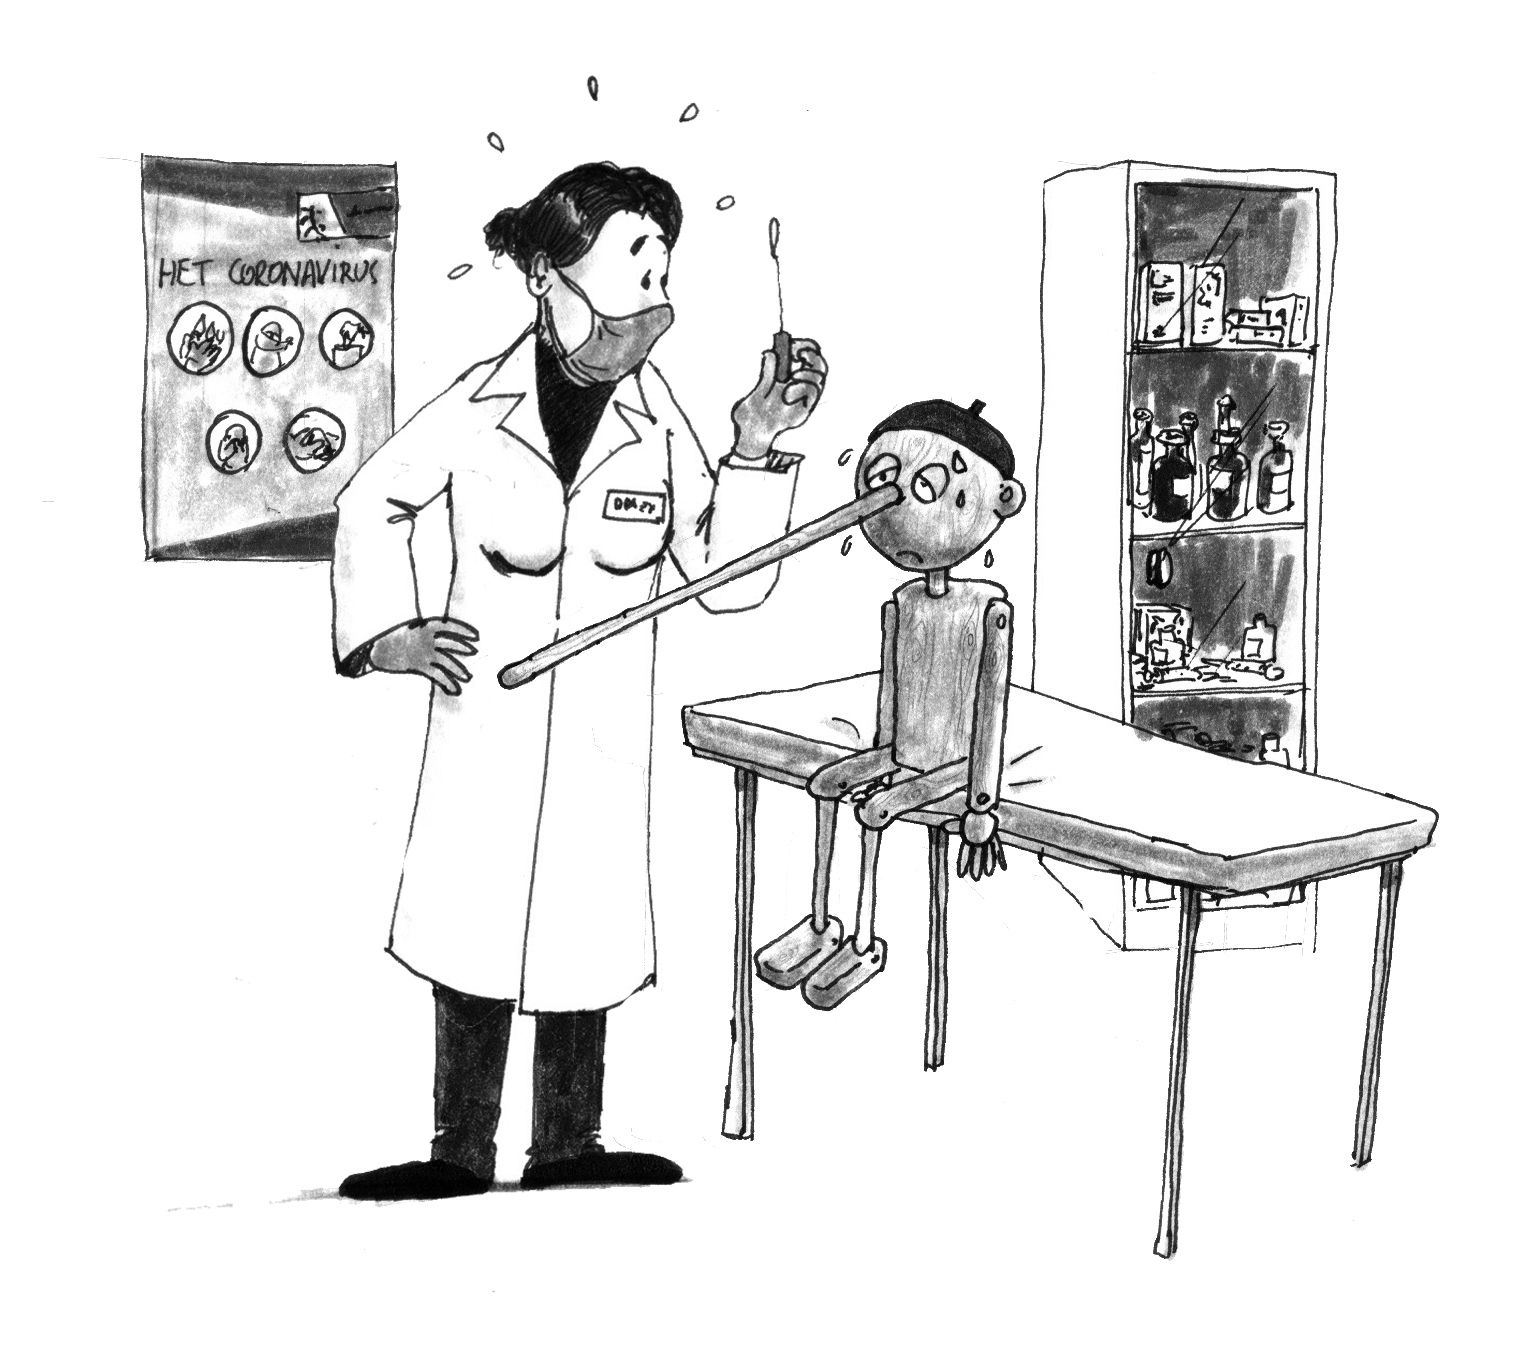
\includegraphics[width=8cm]{img/pinocchio.jpg}
\end{center}
\end{figure}
\vspace{-1cm}

\begin{multicols}{2}
\tussentitel{Besmet of niet: that's the question}
\textbf{Prevalentie} is in het vakjargon de term voor het percentage besmette personen in een populatie. Op de prevalentie van Covid-19 heeft echter niemand momenteel een goed beeld. Geneeskundigen zijn het er over eens dat een grote groep besmette personen enkel milde symptomen of zelfs geen symptomen vertoont. Dat maakt het lastiger om het exacte aantal besmettingen te bepalen. De medische wereld gaat intussen uit van een prevalentie die van maart tot april 2020 hier in België ongeveer 3\% bedroeg.

We passen nu de informatie over de sensitiviteit en specificiteit van de Covid-19-test en de Covid-19-prevalentie toe op een groep van 100 000 Belgen. Per 100 000 inwoners zijn er 3 000 besmettingen.
\begin{center}
\begin{tabular}{|c|
		>{\columncolor[HTML]{FFFFFF}}c |
		>{\columncolor[HTML]{FFFFFF}}c |
		>{\columncolor[HTML]{EFEFEF}}c |}
	\hline
	\textbf{}                               & {\color[HTML]{32CB00} \textbf{Besmet}}                       & {\color[HTML]{FE0000} \textbf{Niet-besmet}}                    & \textbf{Totaal}  \\ \hline
	\cellcolor[HTML]{EFEFEF}\textbf{Totaal} & \cellcolor[HTML]{EFEFEF}{\color[HTML]{32CB00} \textbf{3000}} & \cellcolor[HTML]{EFEFEF}{\color[HTML]{FE0000} \textbf{97 000}} & \textbf{100 000} \\ \hline
\end{tabular}
\end{center}
Wanneer we uitgaan van een sensitiviteit van 71\%, weten we dat 2 130 ($=3 000\cdot0,71$) van de 3 000 besmette personen ook positief zullen testen. De resterende 870 (=$3000\cdot0,29$) besmette personen krijgen verkeerdelijk een negatief testresultaat te zien. Indien de specificiteit 98\% bedraagt, zullen 1 940 (=97 000$\cdot$0,02) niet-besmette personen verkeerdelijk positief testen en de overige 95 060 (=970 000$\cdot$0,98) niet-besmette personen testen terecht negatief. We vatten deze informatie samen in een kruistabel en een boomdiagram. Merk op dat in de takken van het boomdiagram waar de kleur verandert (voor wie dit op de website in kleur bekijkt), er een vals negatief of vals positief resultaat optreedt. In de kruistabel vinden we dit vals negatief en vals positief resultaat terug in de cellen waar de kleur van de kolom niet overeenstemt met de kleur van de rij. 
\end{multicols}
%\vspace{0.5cm}
\begin{center}
	\begin{tabular}{|l|c|c|
			>{\columncolor[HTML]{EFEFEF}}c |}
		\hline
		\multicolumn{1}{|c|}{\textbf{}}                               & \cellcolor[HTML]{FFFFFF}{\color[HTML]{32CB00} \textbf{Besmet}} & \cellcolor[HTML]{FFFFFF}{\color[HTML]{FE0000} \textbf{Niet-besmet}} & \textbf{Totaal}                        \\ \hline
		{\color[HTML]{32CB00} \textbf{Positieve test}}                & {\color[HTML]{32CB00} 2 130}                                   & {\color[HTML]{32CB00} 1 940}                                        & {\color[HTML]{32CB00} \textbf{4 070}}  \\ \hline
		{\color[HTML]{FE0000} \textbf{Negatieve test}}                & {\color[HTML]{FE0000} 870}                                     & {\color[HTML]{FE0000} 95 060}                                       & {\color[HTML]{FE0000} \textbf{95 930}} \\ \hline
		\multicolumn{1}{|c|}{\cellcolor[HTML]{EFEFEF}\textbf{Totaal}} & \cellcolor[HTML]{EFEFEF}{\color[HTML]{32CB00} \textbf{3000}}   & \cellcolor[HTML]{EFEFEF}{\color[HTML]{FE0000} \textbf{97 000}}      & \textbf{100 000}                       \\ \hline
	\end{tabular}

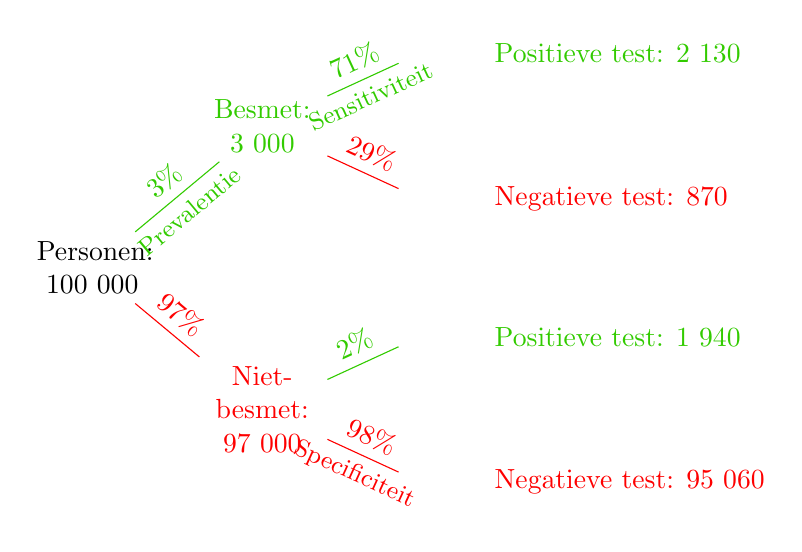
\begin{tikzpicture}[grow=right, sloped,scale=0.8]
\node[bag] {Personen: 100 000}
child[color=red] {
	node[bag] {Niet-besmet: 97 000}        
	child[color=red] {
		node[end, label=right:
		{Negatieve test: 95 060}] {}
		edge from parent
		node[above] {$98\%$}
		node[below]  {\small Specificiteit}
	}
	child[color=green] {
		node[end, label=right:
		{Positieve test: 1 940}] {}
		edge from parent
		node[above] {$2\%$}
		node[below]  {}
	}
	edge from parent 
	node[above] {$97\%$}
	node[below]  {}
}
child[color=green] {
	node[bag] {Besmet: 3 000}        
	child[color=red] {
		node[end, label=right:
		{Negatieve test: 870}] {}
		edge from parent
		node[above] {$29\%$}
		node[below]  {}
	}
	child[color=green] {
		node[end, label=right:
		{Positieve test: 2 130}] {}
		edge from parent
		node[above] {$71\%$}
		node[below]  {\small Sensitiviteit}
	}
	edge from parent         
	node[above] {$3\%$}
	node[below]  {\small{Prevalentie}}
};
\end{tikzpicture}\end{center}


\begin{multicols}{2}
In de realiteit weten we echter niet of iemand besmet is of niet. We willen juist op basis van het testresultaat achterhalen of iemand Covid-19 heeft of niet. De regel van Bayes komt in het spel om de prangende vraag te beantwoorden: `Hoe groot is de kans dat ik besmet ben als mijn Covid-19-test positief is?'. Met andere woorden: wat is de \textit{voorspellende waarde} van een positieve test? Van de 4 070 positief geteste mensen per honderdduizend inwoners (2 130+1 940) zijn er slechts 2 130 effectief besmet, goed voor een percentage van 52,3\% (= 2 130/4 070). \textit{Zelfs met een positieve test in de hand heb je als willekeurige Belg dus slechts de helft kans om effectief besmet te zijn}. Ongeveer 48\% van de positief geteste personen zal een vals positief resultaat krijgen. Zij zullen niet besmet zijn maar zich door het positieve testresultaat waarschijnlijk onnodig zorgen maken.

Conclusie: een prevalentie van 3$\%$ is te laag om iedereen te testen met de huidige generatie PCR-testen. Het aantal vals positieven zou te groot zijn, wat leidt tot onnodige paniek. De lage sensitiviteit (minstens 29\% wordt niet opgemerkt) kan bovendien tot een vals gevoel van veiligheid leiden. Als deze personen vrolijk beslissen om de maatregelen naast zich neer leggen, denkend dat ze niet besmet zijn, kunnen ze veel mensen aansteken.
\end{multicols}

\tussentitel{Gericht testen}
\ \\
\beginwerktekst{Opgave 2}
\noindent We keren terug naar Carl, die tot de risicogroep behoort. Op basis van een groot onderzoek bij alle teruggekeerden van Ischl weet men dat de prevalentie in deze risicogroep 80\% bedraagt. 
\begin{enumerate}
	\item[a.] Indien zijn testresultaat negatief is, wat is dan de kans dat hij niet besmet is? 
	\item[b.]	Wat was zijn kans op besmetting, indien hij positief getest zou hebben?
\end{enumerate}


\emph{\noindent Je kunt het boomdiagram van Carl ook opstellen zonder er aantallen op te kleven. Door de percentages die je op de takken in de boom tegenkomt (bv. 80\% prevalentie, 71\% sensitiviteit) te vermenigvuldigen, krijg je de kans van mensen die besmet zijn \textbf{én} een positief testresultaat kregen (productregel).}
	\begin{center}
	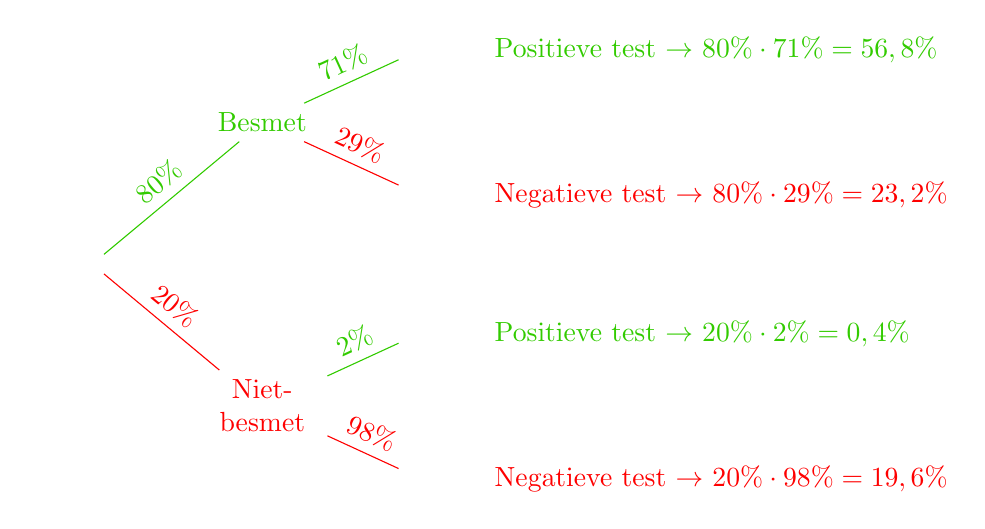
\begin{tikzpicture}[grow=right, sloped,scale=0.8]
	\node[bag] {}
	child[color=red] {
		node[bag] {Niet-besmet}        
		child[color=red] {
			node[end, label=right:
			{Negatieve test $\rightarrow$ $20\%\cdot 98\%=19,6\%$}] {}
			edge from parent
			node[above] {$98\%$}
			node[below]  {}
		}
		child[color=green] {
			node[end, label=right:
			{Positieve test $\rightarrow$ $20\%\cdot 2\% = 0,4\%$}] {}
			edge from parent
			node[above] {$2\%$}
			node[below]  {}
		}
		edge from parent 
		node[above] {$20\%$}
		node[below]  {}
	}
	child[color=green] {
		node[bag] {Besmet}        
		child[color=red] {
			node[end, label=right:
			{Negatieve test $\rightarrow$ $80\%\cdot 29\%= 23,2\%$}] {}
			edge from parent
			node[above] {$29\%$}
			node[below]  {}
		}
		child[color=green] {
			node[end, label=right:
			{Positieve test $\rightarrow$ $80\%\cdot 71\%=56,8\%$}] {}
			edge from parent
			node[above] {$71\%$}
			node[below]  {}
		}
		edge from parent         
		node[above] {$80\%$}
		node[below]  {}
	};
	\end{tikzpicture}
\end{center}
\emph{\begin{enumerate}
	\item[a.] 	In 42,8\% van de gevallen (=\  23,2\%$\ +\ $19,6\%) zal er negatief getest worden, maar slechts 19,6\% zal terecht negatief testen. Carl heeft bij een negatief testresultaat dus maar 45,8\% (= 19,6\%$\ /\ $42,8\%) kans om niet besmet te zijn! Zelfs bij een negatief testresultaat blijft het dus erg waarschijnlijk dat Carl toch besmet is geraakt met Covid-19 tijdens zijn ski-vakantie. 
	\item[b.]Indien Carl positief test, dan is de kans op besmetting zeer groot; we bekomen een predictieve waarde van maar liefst 99,3\% (= 56,8\% / (56,8\% + 0,4\%))! 
\end{enumerate}}
\eindewerktekst
\begin{multicols}{2}

Uit opgave 2, vraag b  blijkt dat een hoge prevalentie de predictieve waarde van een test de hoogte in jaagt: bij een risicogroep met prevalentie van 80$\%$ stijgt ze na een positieve test door naar een kans op besmetting van meer dan 99\%. We moeten vooral de verdachte gevallen gericht testen: mensen die duidelijke ziektesymptomen vertonen, met besmette mensen in contact kwamen of uit een risicogebied komen. Als die positief testen, is een besmetting ook zeer waarschijnlijk. En zolang we alle Covid-19-maatregelen naleven, zijn lang niet alle Belgen verdacht. Iedereen massaal testen heeft dan geen zin en dat is eigenlijk een grote geruststelling.

\tussentitel{Een functie met de prevalentie als onbekende}De prevalentie is in dit verhaal van cruciaal belang, maar tegelijkertijd ook de grote onbekende. Niemand heeft op dit moment enig zicht op de prevalentie van Covid-19. Het is wachten tot betrouwbare steekproefonderzoeken hier hun licht op schijnen. De prevalentie is de \textit{pretestwaarschijnlijkheid}: de kans op besmetting afhankelijk van de groep waartoe men behoort, zonder getest te zijn. De predictieve waarde na een positieve test (de kans op besmetting, gegeven een positief testresultaat) is een \textit{posttestwaarschijnlijkheid}. We kunnen de pretest- en posttestwaarschijnlijkheid uitzetten op een grafiek. Als we $x$ als prevalentie (pretestwaarschijnlijkheid) nemen, opnieuw uitgaande van 0,71 sensitiviteit en 0,98 specifiteit, dan kun je uit de kansboom het functievoorschrift halen van de functie $p_{PCR}:[0,1]\to[0,1]$ die de predictieve waarde (posttestwaarschijnlijkheid) berekent op basis van $x$.
\end{multicols}
\vspace{0.5cm}
\begin{center}
	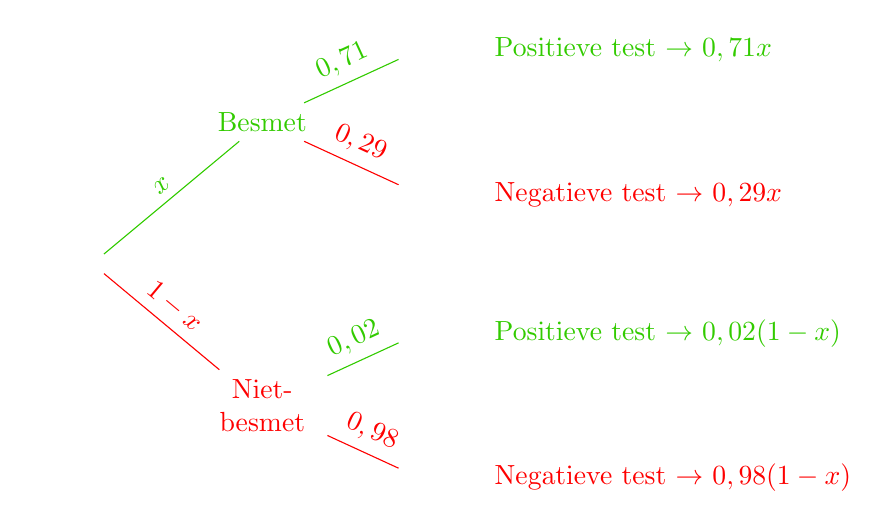
\begin{tikzpicture}[grow=right, sloped,scale=0.8]
	\node[bag] {}
	child[color=red] {
		node[bag] {Niet-besmet}        
		child[color=red] {
			node[end, label=right:
			{Negatieve test $\rightarrow$ $0,98(1-x)$}] {}
			edge from parent
			node[above] {$0,98$}
			node[below]  {}
		}
		child[color=green] {
			node[end, label=right:
			{Positieve test $\rightarrow$ $0,02(1-x)$}] {}
			edge from parent
			node[above] {$0,02$}
			node[below]  {}
		}
		edge from parent 
		node[above] {$1-x$}
		node[below]  {}
	}
	child[color=green] {
		node[bag] {Besmet}        
		child[color=red] {
			node[end, label=right:
			{Negatieve test $\rightarrow$ $0,29x$}] {}
			edge from parent
			node[above] {$0,29$}
			node[below]  {}
		}
		child[color=green] {
			node[end, label=right:
			{Positieve test $\rightarrow$ $0,71x$}] {}
			edge from parent
			node[above] {$0,71$}
			node[below]  {}
		}
		edge from parent         
		node[above] {$x$}
		node[below]  {}
	};
	\end{tikzpicture}
\end{center}
\begin{multicols}{2}
Alle positief geteste gevallen vormen samen $0,71x+0,02(1-x)$. Binnen deze groep vormt $0,71x$ het aandeel van besmette personen dat (terecht) positief test. De predictieve waarde of posttestwaarschijnlijkheid (i.e. de kans op besmetting indien het testresultaat positief is) bedraagt dan:
$$p_{PCR}(x) = \frac{0,71x}{0,71x+0,02(1-x)}.$$
\end{multicols}
\beginwerktekst{Opdracht 3}\\
Zoek het functievoorschrift van de functie $n_{PCR}$, die voor elke prevalentie $x$, de posttestwaarschijnlijkheid geeft bij een negatief testresultaat. $n_{PCR}(x)$ drukt de kans om toch besmet te zijn na een negatieve test bij een prevalentie $x$.\\

\noindent \textit{Antwoord}\\
$$n_{PCR}(x) = \frac{0,29x}{0,29x + 0,98(1-x)}.$$
\eindewerktekst






\begin{multicols}{2}
Figuur \ref{graf1} toont de grafieken van de functies $p_{PCR}$ en $n_{PCR}$.  Merk op dat bij een prevalentie van 20\% de predictieve waarde $p_{PCR}$ al doorstijgt tot 90\%. De rechte $y=x$ toont de theoretische situatie waarbij de test geen extra informatie zou opleveren. In dat geval is de pretestwaarschijnlijkheid even groot als de posttestwaarschijnlijkheid, de test reproduceert gewoon de prevalentie. Het verschil tussen de grafieken van $p_{PCR}$ en $n_{PCR}$ enerzijds en de rechte $y=x$ anderzijds, is een maat voor de extra informatie die de test oplevert.

\end{multicols}
\begin{figure}[t]
	\centering\begin{center}
		\begin{tikzpicture}[line cap=round,line join=round,>=triangle 45,x=10.0cm,y=10.0cm]
		\begin{axis}[
		x=7.0cm,y=7.0cm,
		axis lines=middle,
		ymajorgrids=true,
		xmajorgrids=true,
		xmin=-0.011820689924753836,
		xmax=1.050726146094551958,
		ymin=-0.01931807793339951,
		ymax=1.05148595171747783,
		xtick={-0.1,0.0,...,1.1},
		ytick={-0.0,0.1,...,1.1},
		x label style={at={(axis description cs:0.5,-0.06)},anchor=north},
		y label style={at={(axis description cs:-0.08,.5)},rotate=90,anchor=south},
		xlabel={$x$ pretestwaarschijnlijkheid},
		ylabel={$y$ posttestwaarschijnlijkheid}]
		\clip(-0.11820689924753836,-0.07931807793339951) rectangle (1.0726146094551958,1.0548595171747783);
		\draw[line width=2.pt,color=green,smooth,samples=100,domain=-0.11820689924753836:1.0726146094551958] plot(\x,{(0.71*(\x))/((1.0-(\x))*0.02+0.71*(\x))});
		\draw[line width=2.pt,color=red,smooth,samples=100,domain=-0.11820689924753836:1.0726146094551958] plot(\x,{(0.29*(\x))/(0.29*(\x)+0.98*(1.0-(\x)))});
		\draw [line width=2.pt,dotted,domain=-0.11820689924753836:1.0726146094551958] plot(\x,{(-0.--1.*\x)/1.});
		\begin{scriptsize}
		\draw[color=green] (0.1, 0.92) node {$p_{PCR}$};
		\draw[color=red] (0.45,0.11) node {$n_{PCR}$};
		\draw[color=black] (0.73, 0.83) node {$y=x$};
		\end{scriptsize}
		\end{axis}
		\end{tikzpicture}
	\end{center}
	\caption{Grafieken van de functies $p_{PCR}$ (kans op besmetting bij een positief testresultaat) en $n_{PCR}$ (kans op besmetting bij een negatief testresultaat) voor een Covid-19-test met sensitiviteit van 71\% en specificiteit van 98\%}
	\label{graf1}
\end{figure}
%\begin{multicols}{2}
%\end{multicols}
\beginwerktekst{Opgave 4}
Welke sensitiviteit en specificiteit van een medische test zou ervoor zorgen dat de pre- en posttestwaarschijnlijkheid gelijk zijn en we dus in het geval terechtkomen dat $y=x$?

%\noindent \textbf{Antwoord}\\
\emph{\noindent Elke test waarbij de sensitiviteit en de specificiteit opgeteld exact 100\% geeft, levert geen extra informatie op. Met andere woorden, een test waarbij de sensitiviteit de complementaire kans is van de specificiteit (bv. sensitiviteit/ specificiteit: 70\%/30\%, 50\%/50\%,…) zorgt ervoor dat posttestwaarschijnlijkheid even groot is als de pretestwaarschijnlijkheid. Ook tests waarbij deze som ongeveer gelijk is aan 100$\%$, zullen weinig extra informatie geven. Je kunt dit nagaan door in het boomdiagram de sensitiviteit $a$ en specificiteit $b$ als onbekenden te nemen. De predictieve waarde na een positieve test $\;\;\frac{ax}{ax + (1-b)(1-x)}\;\;$, moet gelijk zijn aan de prevalentie $x$, waaruit volgt:}
\begin{align*}
 \quad  \frac{ax}{ax + (1-b)(1-x)} = x &\Leftrightarrow ax = x[ax + (1-b)(1-x)]\\
    &\Leftrightarrow a = ax + (1-b)(1-x) \\
    &\Leftrightarrow a = ax + 1-x - b + bx\\
    &\Leftrightarrow a - ax + b - bx = 1-x\\
    &\Leftrightarrow a(1-x) + b(1-x) = 1-x\\
    &\Leftrightarrow a + b = 1
\end{align*}
\emph{Dit moet gelden voor elke mogelijk prevalentie $x \in [0,1]$ dus\ $a + b = 1$}
\\
\eindewerktekst

\begin{multicols}{2}
\tussentitel{Gecombineerd testen in het ziekenhuis}
De meeste ziekenhuizen zijn op dit moment opgedeeld in een Covid- en Niet-Covidzone. Elke opgenomen patiënt in een ziekenhuis ondergaat een PCR-test om zo triage mogelijk te maken en Covidpatiënten van andere te scheiden. PCR-testen zijn niet perfect betrouwbaar en het resultaat laat op zich wachten omdat de test eerst naar het labo moet. Daarom wordt er bij elke patiënt meteen een CT (\textit{computed tomography})-check up van de longen gedaan door de radioloog. Je gaat als patiënt even onder de scanner en de radioloog velt op basis van het onderzoek van de longen een oordeel over jouw besmetting. De sensitiviteit en specificiteit van deze CT-test varieert van radioloog tot radioloog, maar gemiddeld genomen rapporteert de wetenschappelijke literatuur een sensitiviteit van 96\% en een erg lage specificiteit van ongeveer 25\%. De lage specificiteit heeft te maken met voorzichtigheid (een radioloog wil zich enkel uitspreken over een niet-besmetting als hij hier echt zeker van is), maar ook vooral omdat elke virale longontsteking er op zo’n CT-scan hetzelfde uitziet: influenza, Covid-19, zware verkoudheden,... zijn niet te onderscheiden.

Het is verleidelijk om de kansen te berekenen van dit gecombineerd testen. We doen dit opnieuw voor willekeurige Belgen en gaan weer uit van een prevalentie van $3\%$. We mogen aannemen dat het resultaat van de CT-testen  onafhankelijk is van het resultaat van de Covid-19-PCR-testen, vermits beide testen onafhankelijk van elkaar afgenomen worden. We stellen het boomdiagram op:
\end{multicols}
\tikzstyle{level 1}=[level distance=2.7cm, sibling distance=4.5cm]
\tikzstyle{level 2}=[level distance=2.5cm, sibling distance=2.3cm]
\tikzstyle{level 3}=[level distance=2.4cm, sibling distance=1.3cm]
% Define styles for bags and leafs
\tikzstyle{bag} = [text width=4em, text centered]
\tikzstyle{end} = [text width=4em, text centered]
\tikzstyle{final} = [circle, minimum width=3pt,fill, inner sep=0pt]
\begin{center}
	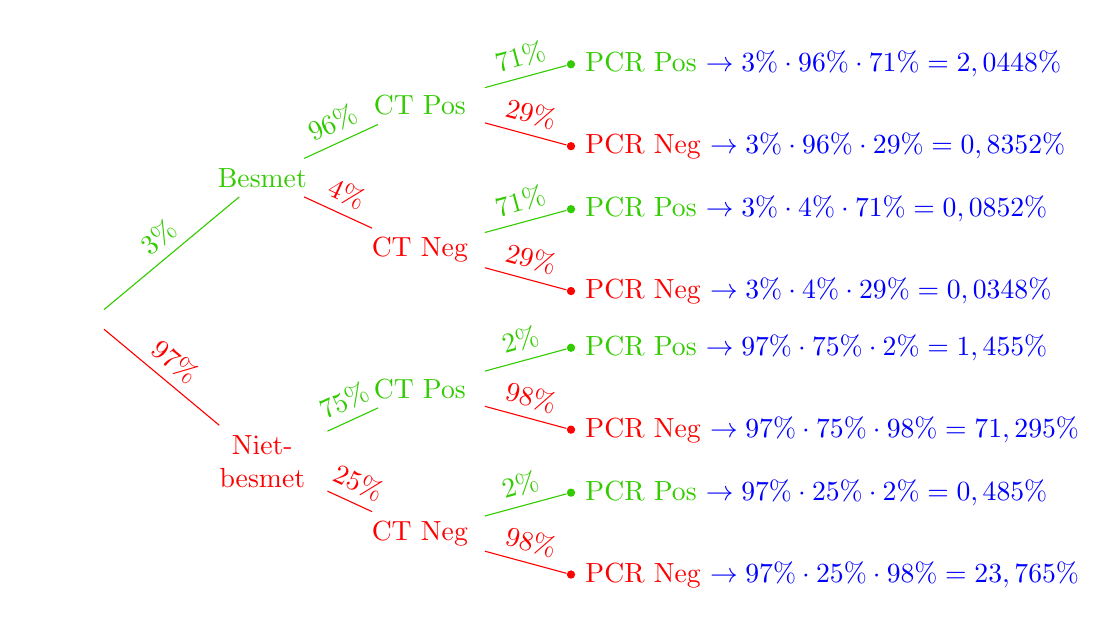
\begin{tikzpicture}[grow=right, sloped,scale=0.8]
	\node[bag] {}
	child[color=red] {
		node[bag] {Niet-besmet}        
		child[color=red] {
			node[end, label=right:] {CT Neg}
			child[color=red]{
				node[final, label=right:{PCR Neg \textcolor{blue}{	$\to 97\%\cdot 25\%\cdot 98\% = 23,765\%$}}]{}
				edge from parent
				node[above] {$98\%$}
				node[below]  {}
			}
			child[color=green]{
				node[final, label=right:{PCR Pos \textcolor{blue}{$\to 97\%\cdot 25\%\cdot 2\% = 0,485\%$}}]{}
				edge from parent
				node[above] {$2\%$}
				node[below]  {}
			}
			edge from parent
			node[above] {$25\%$}
			node[below]  {}
		}
		child[color=green] {
			node[end, label=right:] {CT Pos}
			child[color=red]{
				node[final, label=right:{PCR Neg \textcolor{blue}{$\to 97\%\cdot 75\%\cdot 98\% = 71,295\%$}}]{}
				edge from parent
				node[above] {$98\%$}
				node[below]  {}
			}
			child{
				node[final, label=right:{PCR Pos \textcolor{blue}{$\to 97\%\cdot 75\%\cdot 2\% = 1,455\%$}}]{}
				edge from parent
				node[above] {$2\%$}
				node[below]  {}
			}   
			edge from parent
			node[above] {$75\%$}
			node[below]  {}
		}
		edge from parent 
		node[above] {$97\%$}
		node[below]  {}
	}
	child[color=green] {
		node[bag] {Besmet}        
		child[color=red] {        	
			node[end, label=right:] {CT Neg}
			child{
				node[final, label=right:{PCR Neg \textcolor{blue}{$\to 3\%\cdot 4\%\cdot 29\% = 0,0348\%$}}]{}
				edge from parent
				node[above] {$29\%$}
				node[below]  {}
			}
			child[color=green]{
				node[final, label=right:{PCR Pos \textcolor{blue}{$\to 3\%\cdot 4\%\cdot 71\% = 0,0852\%$}}]{}
				edge from parent
				node[above] {$71\%$}
				node[below]  {}
			}
			edge from parent
			node[above] {$4\%$}
			node[below]  {}
		}
		child[color=green] {
			node[end, label=right:] {CT Pos}
			child[color=red]{
				node[final, label=right:{PCR Neg \textcolor{blue}{$\to 3\%\cdot 96\%\cdot 29\% = 0,8352\%$}}]{}
				edge from parent
				node[above] {$29\%$}
				node[below]  {}
			}
			child{
				node[final, label=right:{PCR Pos \textcolor{blue}{$\to 3\%\cdot 96\%\cdot 71\% = 2,0448\%$}}]{}
				edge from parent
				node[above] {$71\%$}
				node[below]  {}
			}   
			edge from parent
			node[above] {$96\%$}
			node[below]  {}
		}
		edge from parent         
		node[above] {$3\%$}
		node[below]  {}
	};
	\end{tikzpicture}
\end{center}
\begin{multicols}{2}

Wat is de kans op besmetting als iemand zowel een positieve CT-scan als een positieve Covid-19-PCR-test heeft gekregen? De kans op twee positieve testen bedraagt 2,0448\% + 1,455\% = 3,4998\%. De kans op besmetting indien iemand voor elk van deze testen een positief resultaat behaalde, is gelijk aan 58,4\% (= 2,0448\%/3,4998\%). Dit resultaat valt tegen aangezien het niet veel verschilt van de voorspellende waarde van de PCR-test alleen (nl. $52,3\%$). Bovendien verwatert het effect van gecombineerd testen nog verder als we uitgaan van een hogere prevalentie (zie opgave 5). Merk op dat een prevalentie hoger dan 3\% ook best mogelijk is in een ziekenhuis-context, aangezien mensen die zich aanmelden in het ziekenhuis niet zomaar willekeurige Belgen zijn, maar zieke mensen, waarvan een groot deel expliciete Covid-klachten heeft.
\end{multicols}

\beginwerktekst{Opgave 5}
Veronderstel dat de prevalentie 60$\%$ bedraagt bij mensen die zich in het ziekenhuis aanmelden met mogelijke Covid-19. Hoe groot is de kans dat iemand besmet is bij (a) 2 positieve testen (zowel CT als Covid-19 PCR) en (b) de Covid-19-PCR-test alleen?
		
%\noindent \textbf{Antwoord}\\
\emph{\noindent (a) 98,5\% ; (b) 98,2\%.}\\
\eindewerktekst
\begin{figure}[H]
	\centering\begin{center}
		\begin{tikzpicture}[line cap=round,line join=round,>=triangle 45,x=5.0cm,y=5.0cm]
		\begin{axis}[
		x=7.0cm,y=7.0cm,
		axis lines=middle,
		ymajorgrids=true,
		xmajorgrids=true,
		xmin=-0.011820689924753836,
		xmax=1.050726146094551958,
		ymin=-0.01931807793339951,
		ymax=1.05148595171747783,
		xtick={-0.1,0.0,...,1.1},
		ytick={-0.0,0.1,...,1.1},
		x label style={at={(axis description cs:0.5,-0.06)},anchor=north},
		y label style={at={(axis description cs:-0.08,.5)},rotate=90,anchor=south},
		xlabel={$x$ pretestwaarschijnlijkheid},
		ylabel={$y$ posttestwaarschijnlijkheid}]
		\clip(-0.11820689924753836,-0.07931807793339951) rectangle (1.0726146094551958,1.0548595171747783);
		\draw[line width=2.pt,color=green,smooth,samples=100,domain=-0.11820689924753836:1.0726146094551958] plot(\x,{(0.96*(\x))/((1.0-(\x))*0.75+0.96*(\x))});
		\draw[line width=2.pt,color=red,smooth,samples=100,domain=-0.11820689924753836:1.0726146094551958] plot(\x,{(0.04*(\x))/(0.04*(\x)+0.25*(1.0-(\x)))});
		\draw [line width=2.pt,dotted,domain=-0.11820689924753836:1.0726146094551958] plot(\x,{(-0.--1.*\x)/1.});
		\begin{scriptsize}
		\draw[color=green] (0.1, 0.18) node {$p_{CT}$};
		\draw[color=red] (0.2,0.08) node {$n_{CT}$};
		\draw[color=black] (0.74, 0.65) node {$y=x$};
		\end{scriptsize}
		\end{axis}
		\end{tikzpicture}
	\end{center}
	\caption{Grafieken van de functies $p_{CT}$ en $n_{CT}$}
	\label{graf2}
\end{figure}
\begin{multicols}{2}

\noindent Uit opgave 4 weten we dat een medische test, waarvan de sensitiviteit en specificiteit samen ongeveer 100\% geven, weinig extra informatie zal geven. Als we de sensitiviteit en de specificiteit van de CT-test optellen, komen we aan 121\%, dat is niet veel verwijderd van 100\%. De beperkte meerwaarde van de CT-test bij het detecteren van Covid-19 is grafisch duidelijk als we de functies $p_{CT}$ (kans op besmetting na een positieve CT-test) en $n_{CT}$ (kans op besmetting na een negatieve CT-test) uitzetten (zie figuur \ref{graf2}). 


 De grafiek van de functie $p_{CT}$ leunt dicht aan bij de grafiek van $y=x$, wat betekent dat na een positieve CT-test, de kans op besmetting slechts een klein beetje hoger is dan de initiële prevalentie. Merk op dat de extra informatie vooral zit in de functie $n_{CT}$: iemand met een negatieve CT-scan, heeft effectief een veel lagere besmettingskans dan de prevalentie. Door de lage specificiteit, zullen weinig patiënten een negatieve CT-test krijgen (25\%), maar diegene die toch met een negatieve CT-test naar buiten lopen, mogen vrij gerust zijn.\textit{ Dat is een constante in de medische wereld: de eerste test (bv. CT) is meestal heel sensitief, maar heel weinig specifiek. De tweede test (bv. PCR) is meestal heel specifiek, maar weinig sensitief.} In het ziekenhuis worden patiënten met een negatieve CT-test ook opgenomen op een afdeling met niet-besmette patiënten. Voor diegene met een positieve CT-scan, maar een negatieve PCR-test, wordt er na 24u opnieuw een PCR-test uitgevoerd: de virale lading kan gewijzigd zijn en daardoor het testresultaat meer betrouwbaar maken.


\tussentitel{Een toekomst voor immuniteitstesten?}
Om het normale leven terug op gang te trekken, adviseren denktanks om mensen een immuniteitstest te laten ondergaan vooraleer ze weer aan het werk mogen. Deze serologische test zoekt in het bloed naar antilichamen tegen Covid-19 en verschilt fundamenteel van de PCR-test. Die gaat enkel ‘besmetting’ na, terwijl een serologische test nagaat of er antilichamen zijn aangemaakt. De gerapporteerde sensitiviteit van de immuniteitstest die in de Verenigde Staten wordt gebruikt, bedraagt 93,8\% en de specificiteit 95,6\%. Er zit wel een addertje onder het gras: je kunt Covid-19 hebben doorgemaakt maar toch geen immuniteit hebben opgebouwd (of deze immuniteit na verloop van tijd verloren zijn) en ook omgekeerd: je kunt immuniteit hebben opgebouwd, maar nog altijd drager zijn van het virus en zo mensen besmetten. Daarom wordt aangeraden om iedereen die positief test op de immuniteitstest, ook te testen met PCR-test, die dan een negatief resultaat moet opleveren. Hoewel we zouden willen, is het op het moment van dit schrijven onmogelijk om de gecombineerde kansen hiervan in te schatten. Je moet de bevolking immers opdelen in vier groepen: WEL immuun/WEL besmettelijk, WEL immuun/NIET besmettelijk, NIET immuun/WEL besmettelijk en NIET immuun/NIET besmettelijk. We hebben al geen betrouwbaar idee van de prevalentie van Covid-19, laat staan dat we zouden weten hoe die groepen zich onderling verhouden. Zonder enig zicht hierop, lijkt deze teststrategie voorlopig gebaseerd op drijfzand... To be continued!

\tussentitel{Conclusie}
Medische tests zijn nooit 100\% betrouwbaar. Na een negatief testresultaat is er steeds een reële kans op besmetting en vice versa. Bovendien worden deze kansen sterk beïnvloed door de prevalentie van een ziekte (bv. Covid-19). Het subtiele samenspel tussen pretestwaarschijnlijkheid en posttestwaarschijnlijkheid kan mooi grafisch uitgezet worden. Als we ervoor zorgen dat het coronavirus zich niet massaal verspreidt onder de Belgische bevolking, is het overbodig om iedereen te testen: het aantal vals positieven zou de pan uit swingen en vele mensen onnodig ongerust maken. Anderzijds is het gericht testen van verdachte gevallen noodzakelijk om het virus te lijf te gaan en kan ook gecombineerd testen misschien een uitweg uit deze crisis bieden. 





\section{Een onderzoeksproject rond het VAN-model}

Bij de uitbraak van de corona-epidemie weerklonk in de geschreven en gesproken pers voortdurend de slogan: `flatten the curve'. Met deze leuze trachtten de virologen de bevolking aan te manen de onderlinge fysieke contacten te beperken zodanig dat de top in de infectiegrafiek zou kunnen zakken en vooruitgeschoven zou worden in de tijd. Dit eerste was nodig om een overbelasting van de intensieve verzorging in de ziekenhuizen te voorkomen. Het tweede zorgde voor een extra voorbereidingstijd voor de ziekenhuizen. De gezondheidszorg was immers slecht voorbereid op de snelheid waarmee de epidemie zich uitbreidde.

Tijdens de lockdown besloten mijn collega en ik een seminarieproject te wijden aan de verspreiding van infectiezieken om op deze manier beter te kunnen begrijpen hoe het afvlakken van de curve precies werkte. We deden dit met onze leerlingen van 5 en 6 wetenschappen-wiskunde en Latijn-wiskunde. Bij het modelleren kozen we voor het SIR-algoritme, dat ook volop aandacht kreeg in de pers. In onze versie vertaalden we deze benaming tot het VAN-algoritme, refererend aan de drie klassen waarin de bevolking wordt ingedeeld: V voor de klasse van de \textbf{v}atbare personen, A voor de \textbf{a}angetaste personen en N voor de \textbf{n}iet meer besmette personen (genezen verklaard of gestorven).

We startten onze lessen met een snelcursus programmeren. Hierbij kozen we voor het gratis cloudprogramma CoCalc, dat werkt met een Pythonachtige programmeertaal. Deze snelcursus vind je op de website van Uitwiskeling. 

Nadien stelden we een tekst op over basisprincipes van het VAN-algoritme. Deze tekst eindigt met opdrachten die de leerling op weg zetten naar geschikte onderzoeksvragen. Gaat de top van de infectiegrafiek altijd naar omlaag als de hygiënische voorzorgsmaatregelen goed opgevolgd worden? Wordt deze top altijd uitgesteld in de tijd als we veiliger leven? Wanneer gaat een epidemisch verloop over in een uitdovende ziekte? ... Ook deze tekst vind je op de website van Uitwiskeling. 

Het doel van dit onderzoeksproject was: leren modelleren, programmeren, analyseren en rapporteren. Dit laatste was het belangrijkste. In het verslag mochten de leerlingen deeltjes overnemen uit de basistekst over het VAN-algoritme en moesten ze ook hun eigen ontdekkingen toevoegen. De bedoeling was een tekst te produceren die zonder bijkomende uitleg begrijpbaar was voor leerlingen van een parallelklas. Vooral de leerlingen van het vijfde jaar hadden het moeilijk met het schrijven van duidelijke teksten. Daarom besloten we het verslag te laten maken in een gedeeld document. Zo kon de leerkracht makkelijk tussentijdse correcties maken en kon hij zo nodig suggesties in  het chatvenster schrijven. Meer nog dan in het zesde jaar is het verslag van de leerlingen van het vijfde jaar ontstaan met de leerkracht als co-auteur. Deze begeleiding tijdens het schrijfproces zorgde voor een positief gevoel bij leerlingen die weinig ervaring hadden met het schrijven van een wetenschappelijk verslag.

Voor we verder gaan met de bespreking van het VAN-project, tonen we hieronder een compilatie van de verslagen. We presenteren deze compilatie als een afgewerkte lesactiviteit. Maar we willen duidelijk benadrukken dat er weken door de leerlingen en hun leerkracht aan de tekst is gesleuteld en bijgeschaafd om een leesbare vorm te krijgen. 

\end{multicols}

\subsection{Schriftelijk verslag van het onderzoek}

\beginwerktekst{Het VAN-model voor het verspreiden van infectieziekten}

\tussentitel{De computersimulatie}

In het eerste deel van het project over het verspreiden van infectieziekten schreven we een programma om de fractie vatbare personen $v(t)$, de fractie aangetaste personen $a(t)$ en de fractie niet meer aangetaste personen $n(t)$ van een populatie bij een infectieziekte te voorspellen
met het VAN-model. Om de grootte van deze drie klassen te berekenen gebruikten we de volgende drie \emph{differentievergelijkingen}:

\begin{align}
\Delta v(t)&=-b \cdot v(t) \cdot a(t) \\
\Delta a(t)&=b \cdot v(t) \cdot a(t)-g \cdot a(t) \\
\Delta n(t)&=+g \cdot a(t)
\end{align}

In deze vergelijkingen komen twee constanten voor. De constante $b$ staat voor de \emph{besmettingsgraad} en de constante $g$ voor de \emph{genezingsgraad}. Verder steunen de berekeningen op de beginsituatie die gegeven wordt door de gekozen startwaarden $v(0)$, $a(0)$ en $n(0)$.

De populaties $v(t)$, $a(t)$ en $n(t)$ werden in het computerprogramma stap voor stap berekend met tijdsintervalletjes gelijk aan een kwart van een dag. Zo bekwamen we getrapte grafieken voor de functies $v(t)$, $a(t)$ en $n(t)$. Omdat de trapjes heel klein zijn, lijken de grafieken echter vloeiend te zijn. 

Voor een eerste experiment kozen we een willekeurig besmettings- en genezingsgraad. We stelden dat bij het begin van de infectie slechts $1\%$ van de populatie aangetast was en $99\%$ vatbaar was voor de ziekte. Dit leek een aanvaardbare beginsituatie. Bij de gegevens $b=\frac{1}{15}$, $g=\frac{1}{60}$, $v(0)=\frac{99}{100}$, $a(0)=\frac{1}{100}$ en $n(0)=0$ vonden we dan de volgende grafieken voor de drie populatieklassen. Op de horizontale as lezen we de tijd af in (hele) dagen, op de verticale as de grootte van de drie klassen van de populatie.

\begin{center}
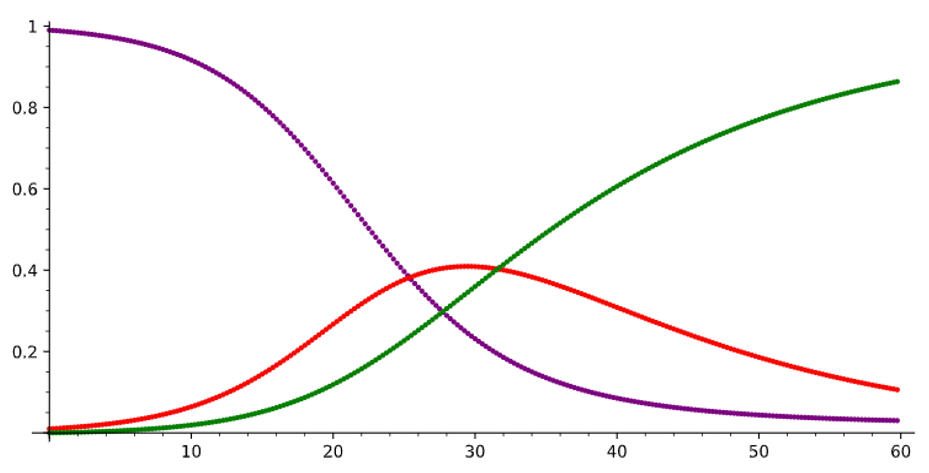
\includegraphics[width=0.7\linewidth]{img/driegrafieken.jpg}
\captionof{figure}{De grafieken van de functies $v(t)$, $a(t)$ en $n(t)$}
\label{driegrafieken}
\end{center}

De dalende grafiek is die van de functie $v(t)$, de stijgende is die van de functie $n(t)$ en de grafiek die eerst stijgt en daarna daalt is die van de infectiefunctie $a(t)$. Grofweg kunnen we zeggen dat na 30 dagen ongeveer 40\% van de bevolking besmet is. Daarna mindert de ziekte in kracht.
\ \\
\ \\


\tussentitel{Eerste vaststelling: de top van de infectiegrafiek}

Stel dat we alle parameters constant houden en dat we alleen de besmettingsgraad $b$ wijzigen, dan kunnen we vaststellen hoe een vermindering van de besmettingsgraad inwerkt op de piek van de besmetting.

We nemen voor de besmettingsgraad achtereenvolgens $b=\frac{1}{5}, b=\frac{1}{10}, b=\frac{1}{15}, \dots, b=\frac{1}{35}$ en $b=\frac{1}{40}$. Visueel stellen we dan vast dat de top van de infectiegrafiek tijdens deze evolutie naar rechts opschuift in de tijd en dat de top ook lager wordt. Door de kans op besmetting te verminderen (bijvoorbeeld via social distancing, het dragen van mondkapjes en het regelmatig ontsmetten van de handen) wordt de druk op de intensieve verzorgingsafdeling van de ziekenhuizen in het piekmoment dus verlicht. De piek wordt ook uitgesteld zo dat er een langere voorbereidingstijd ontstaat vooraleer de piek van het aantal slachtoffers in de ziekenhuizen opgevangen moet worden.

\begin{center}
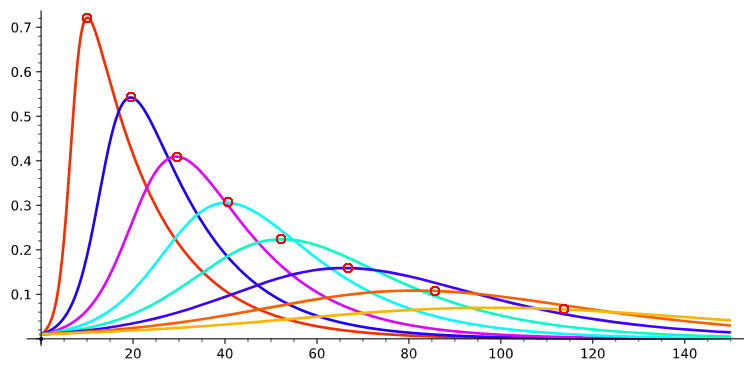
\includegraphics[width=0.8\linewidth]{img/flattenthecurve.jpg}
\captionof{figure}{Afvlakken van de infectiegrafiek}
\label{flatten}
\end{center}

Dit ene voorbeeld bewijst niet dat de top in alle omstandigheden afgevlakt wordt. Om hier een gefundeerde uitspraak over te kunnen doen, moeten we ook extremere waarden voor de besmettingsgraad $b$ onderzoeken, andere genezingsgraden $g$ en andere waarden voor de drie beginpopulaties. 


\tussentitel{Tweede vaststelling: de totale impact van de infectie}

Of de totale impact van de ziekte ook vermindert bij de verkleining van de besmettingsgraad, kunnen we onderzoeken door de oppervlakte onder de infectiegrafiek te berekenen. De oppervlakte onder deze grafiek is evenredig met de totale druk die op de maatschappij rust na het uitbreken van de infectieziekte.  

We geven hiervan een eenvoudig voorbeeld. Een epidemie die twee dagen lang 60\% van de bevolking infecteert, twee dagen lang 50\% van de bevolking, de twee volgende dagen 40\%, daarna 30\% en daarna 20\% heeft dezelfde impact als een epidemie die 10 dagen lang 40\% van de bevolking teistert. De oppervlakte onder beide grafieken is immers gelijk, zie figuur \ref{opp1} en figuur \ref{opp2}. 

\begin{center}
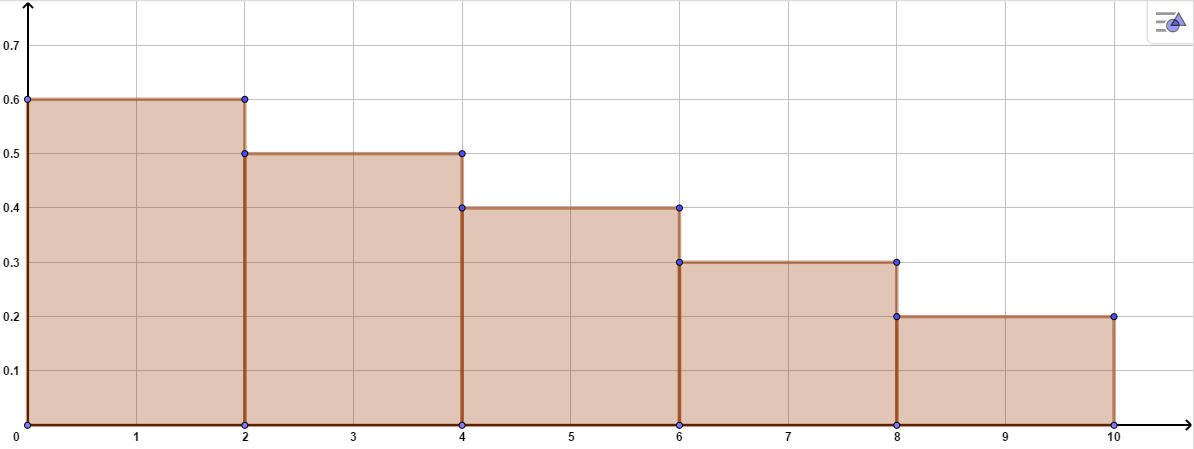
\includegraphics[width=0.65
\linewidth]{img/oppervlakte1.jpg}
\captionof{figure}{Impact van een ziekte met een dalend infectieverloop}
\label{opp1}
\end{center}

\begin{center}
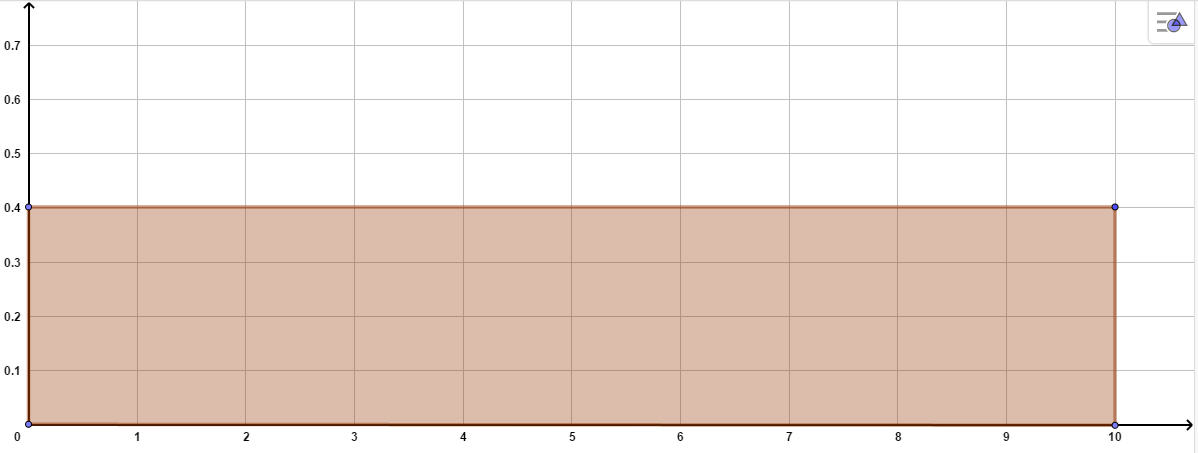
\includegraphics[width=0.65\linewidth]{img/oppervlakte2.jpg}
\captionof{figure}{Impact van een ziekte met een constant infectieverloop}
\label{opp2}
\end{center}

Deze oppervlakte is gelijk aan 4 (met als eenheid: dagen $\times$ procent van de bevolking). Je kan de impact van deze epidemie vergelijken met die van een infectieziekte die gedurende vier dagen de hele bevolking besmet houdt. 

Om de oppervlakte onder de infectiegrafieken te naderen, beschouwen we de grafiek als een trapfunctie. De oppervlakte onder de kromme berekenen we door de oppervlakte van rechthoekjes op te tellen.

Zoals hierboven nemen we opnieuw: $g=\frac{1}{60}$, $v(0)=\frac{99}{100}$, $a(0)=\frac{1}{100}$ en $n(0)=0$ en kiezen we voor de afnemende besmettingsgraden weer $b=\frac{1}{5}, b=\frac{1}{10}, b=\frac{1}{15}, \dots, b=\frac{1}{35}$ en $b=\frac{1}{40}$. De cijfers uit figuur \ref{impact1}  tonen aan dat totale impact van de epidemie afneemt wanneer de besmettingsgraad afneemt.

\begin{center}
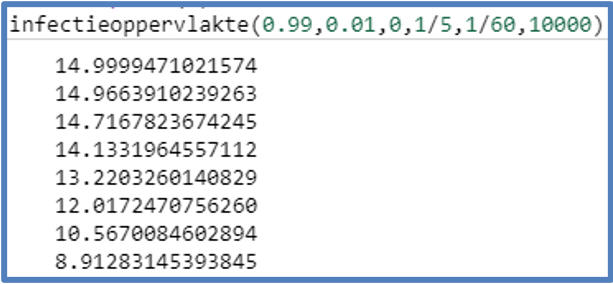
\includegraphics[width=0.6\linewidth]{img/impact1.jpg}
\captionof{figure}{Dalende impact van de epidemie op de maatschappij bij een genezingsgraad $g=\frac{1}{60}$}
\label{impact1}
\end{center}

Voor een lagere genezingsgraad, bijvoorbeeld $g=\frac{1}{100}$, kunnen we eenzelfde conclusie trekken. De afname van de totale impact van de epidemie is echter minder groot volgens de cijfers uit figuur \ref{impact2}.

\begin{center}
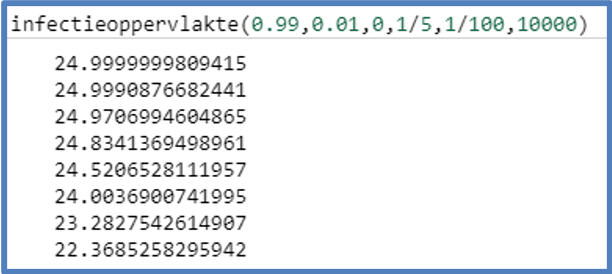
\includegraphics[width=0.6\linewidth]{img/impact2.jpg}
\captionof{figure}{Dalende impact van de epidemie op de maatschappij bij een genezingsgraad $g=\frac{1}{100}$}
\label{impact2}
\end{center}

Voor een grotere genezingsgraad, bijvoorbeeld $g=\frac{1}{40}$, is het effect op de totale impact van de epidemie bij het verminderen van de besmettingsgraad veel sterker.

\begin{center}
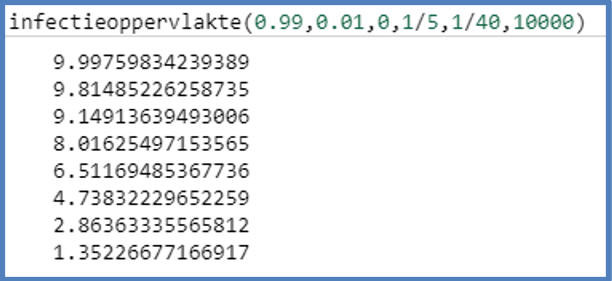
\includegraphics[width=0.6\linewidth]{img/impact3.jpg}
\captionof{figure}{Dalende impact van de epidemie op de maatschappij bij een genezingsgraad $g=\frac{1}{40}$}
\label{impact3}
\end{center}

\tussentitel{Derde vaststelling: de besmettingsgrafiek heeft niet altijd een stijgend verloop}

In het bovenstaande voorbeeld was de infectiegrafiek eerst stijgend en daarna dalend. Soms is de grafiek echter alleen dalend. Om deze  dalende grafieken duidelijker in beeld te krijgen, moeten we extremere waarden geven aan de parameters. Dit kan bijvoorbeeld door een nog kleinere besmettingsgraad te kiezen.

Stel dat bij het begin een honderdste van de populatie geïnfecteerd is: $v(0)=\frac{99}{100}$, $a(0)=\frac{1}{100}$ en $n(0)=0$. Stel ook dat  $g=\frac{1}{60}$. We nemen voor de besmettingsgraden kleinere waarden dan $b=\frac{1}{40}$ uit de vorige simulatie. Stel achtereenvolgens $b=\frac{1}{48}$,$b=\frac{1}{49}$,…, $b=\frac{1}{59}$, $b=\frac{1}{60}$, …, $b=\frac{1}{64}$, $b=\frac{1}{65}$. Dan vinden we de volgende achttien infectiegrafieken.

\begin{center}
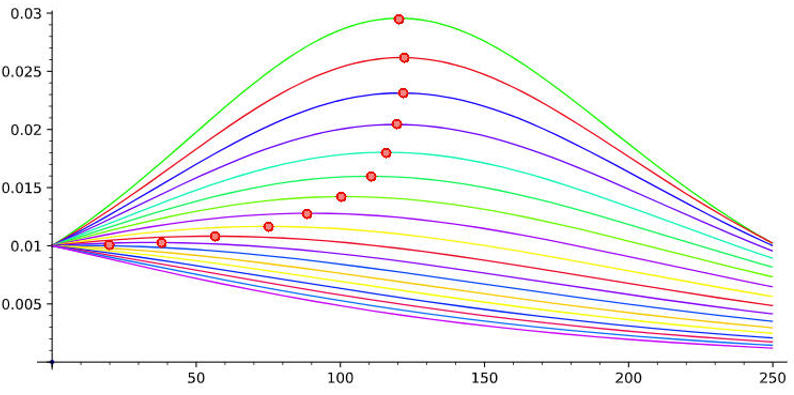
\includegraphics[width=0.8\linewidth]{img/retrograde.jpg}
\captionof{figure}{De top maakt een teruglopende beweging}
\label{retrograde}
\end{center}

We bekijken de grafieken uit figuur \ref{retrograde} van boven naar beneden. De eerste twaalf grafieken hebben een stijgend en dalend verloop. De beweging die de top maakt, verschilt van de beweging die we bij het begin van het onderzoek kregen. De top schuift aanvankelijk naar rechts op in de tijd maar verderop is er een teruglopende beweging. De piek van de infecties neemt in deze laatste fase wel af maar hij komt sneller in de tijd.

De laatste zes grafieken hebben geen stijgend verloop. Het aantal besmette personen neemt alleen maar af. In deze gevallen spreken we niet meer van een epidemie, maar wel van een uitdovende besmettingsziekte.

Bij de overgang van een epidemische ziekte naar een uitdovende besmettingsziekte is er een denkbeeldige  overgangsgrafiek waarbij de top ligt bij $t=0$. Deze overgangsgrafiek is niet getekend op figuur \ref{retrograde}. In het laatste deel van dit verslag onderzoeken we theoretisch waar de omslag ligt van een epidemische naar een uitdovend verloop.

\tussentitel{Vierde vaststelling: het omslagpunt kan theoretisch voorspeld worden}

De overgang van een infectiegrafiek die stijgt en daalt naar een infectiegrafiek die alleen maar dalend is, vinden we bij de grafiek waarbij de raaklijn in het beginpunt $(0, a(0))$ horizontaal is. In een mini-omgeving rechts van deze top zal $a(t)$ ongeveer constant zijn. De differentie $\Delta a(t)$ is er nul. 

We stellen dus dat $\Delta a(t)$ gelijk is aan 0 voor $t=0$. Uit formule (2) vinden we dan dat:
\[\Delta a(0)=+b \cdot v(0) \cdot a(0)-g \cdot a(0)=0.\]
Omdat $a(0) \neq 0$ volgt hieruit dat:
\[b \cdot v(0)-g=0\]
of dat:
\[\frac{b \cdot v(0)}{g}=1.\]

Het getal $\frac{b \cdot v(0)}{g}$ noemen we het basisreproductiegetal. In de medische literatuur wordt dit getal benoemd met het symbool $R_0$. $R_0$ geeft aan hoeveel personen een geïnfecteerde persoon gemiddeld besmet gedurende zijn hele ziekteproces (indien er geen personen  ingeënt zijn of immuun worden). Als een deel van de populatie immuun wordt, verandert het reproductiegetal. We spreken dan van het effectieve reproductiegetal $R$. Tijdens een epidemie verandert het reproductiegetal $R$ van dag tot dag. Is het groter dan 1 dan zijn er drastische maatregelen nodig. Is het kleiner dan 1 dan evolueert de epidemie in goede zin.

Voor de Ebola-epidemie in 2014 werd het basisreproductiegetal geraamd op 1,5 tot 2,5. De luchtwegeninfectie SARS die in 2002 over kwam vanuit China en Hongkong had een basisreproductie getal tussen 2 en 5. Het basisreproductiegetal van Covid-19 lag in dezelfde lijn: tussen 2,4 en 3,9. Mazelen is een uitschieter met $R_0$ tussen 12 en 18. Al deze ziekten zijn erkend als epidemieën omdat het basisreproductiegetal groter is dan 1.

\begin{figure}[H]
\begin{center}
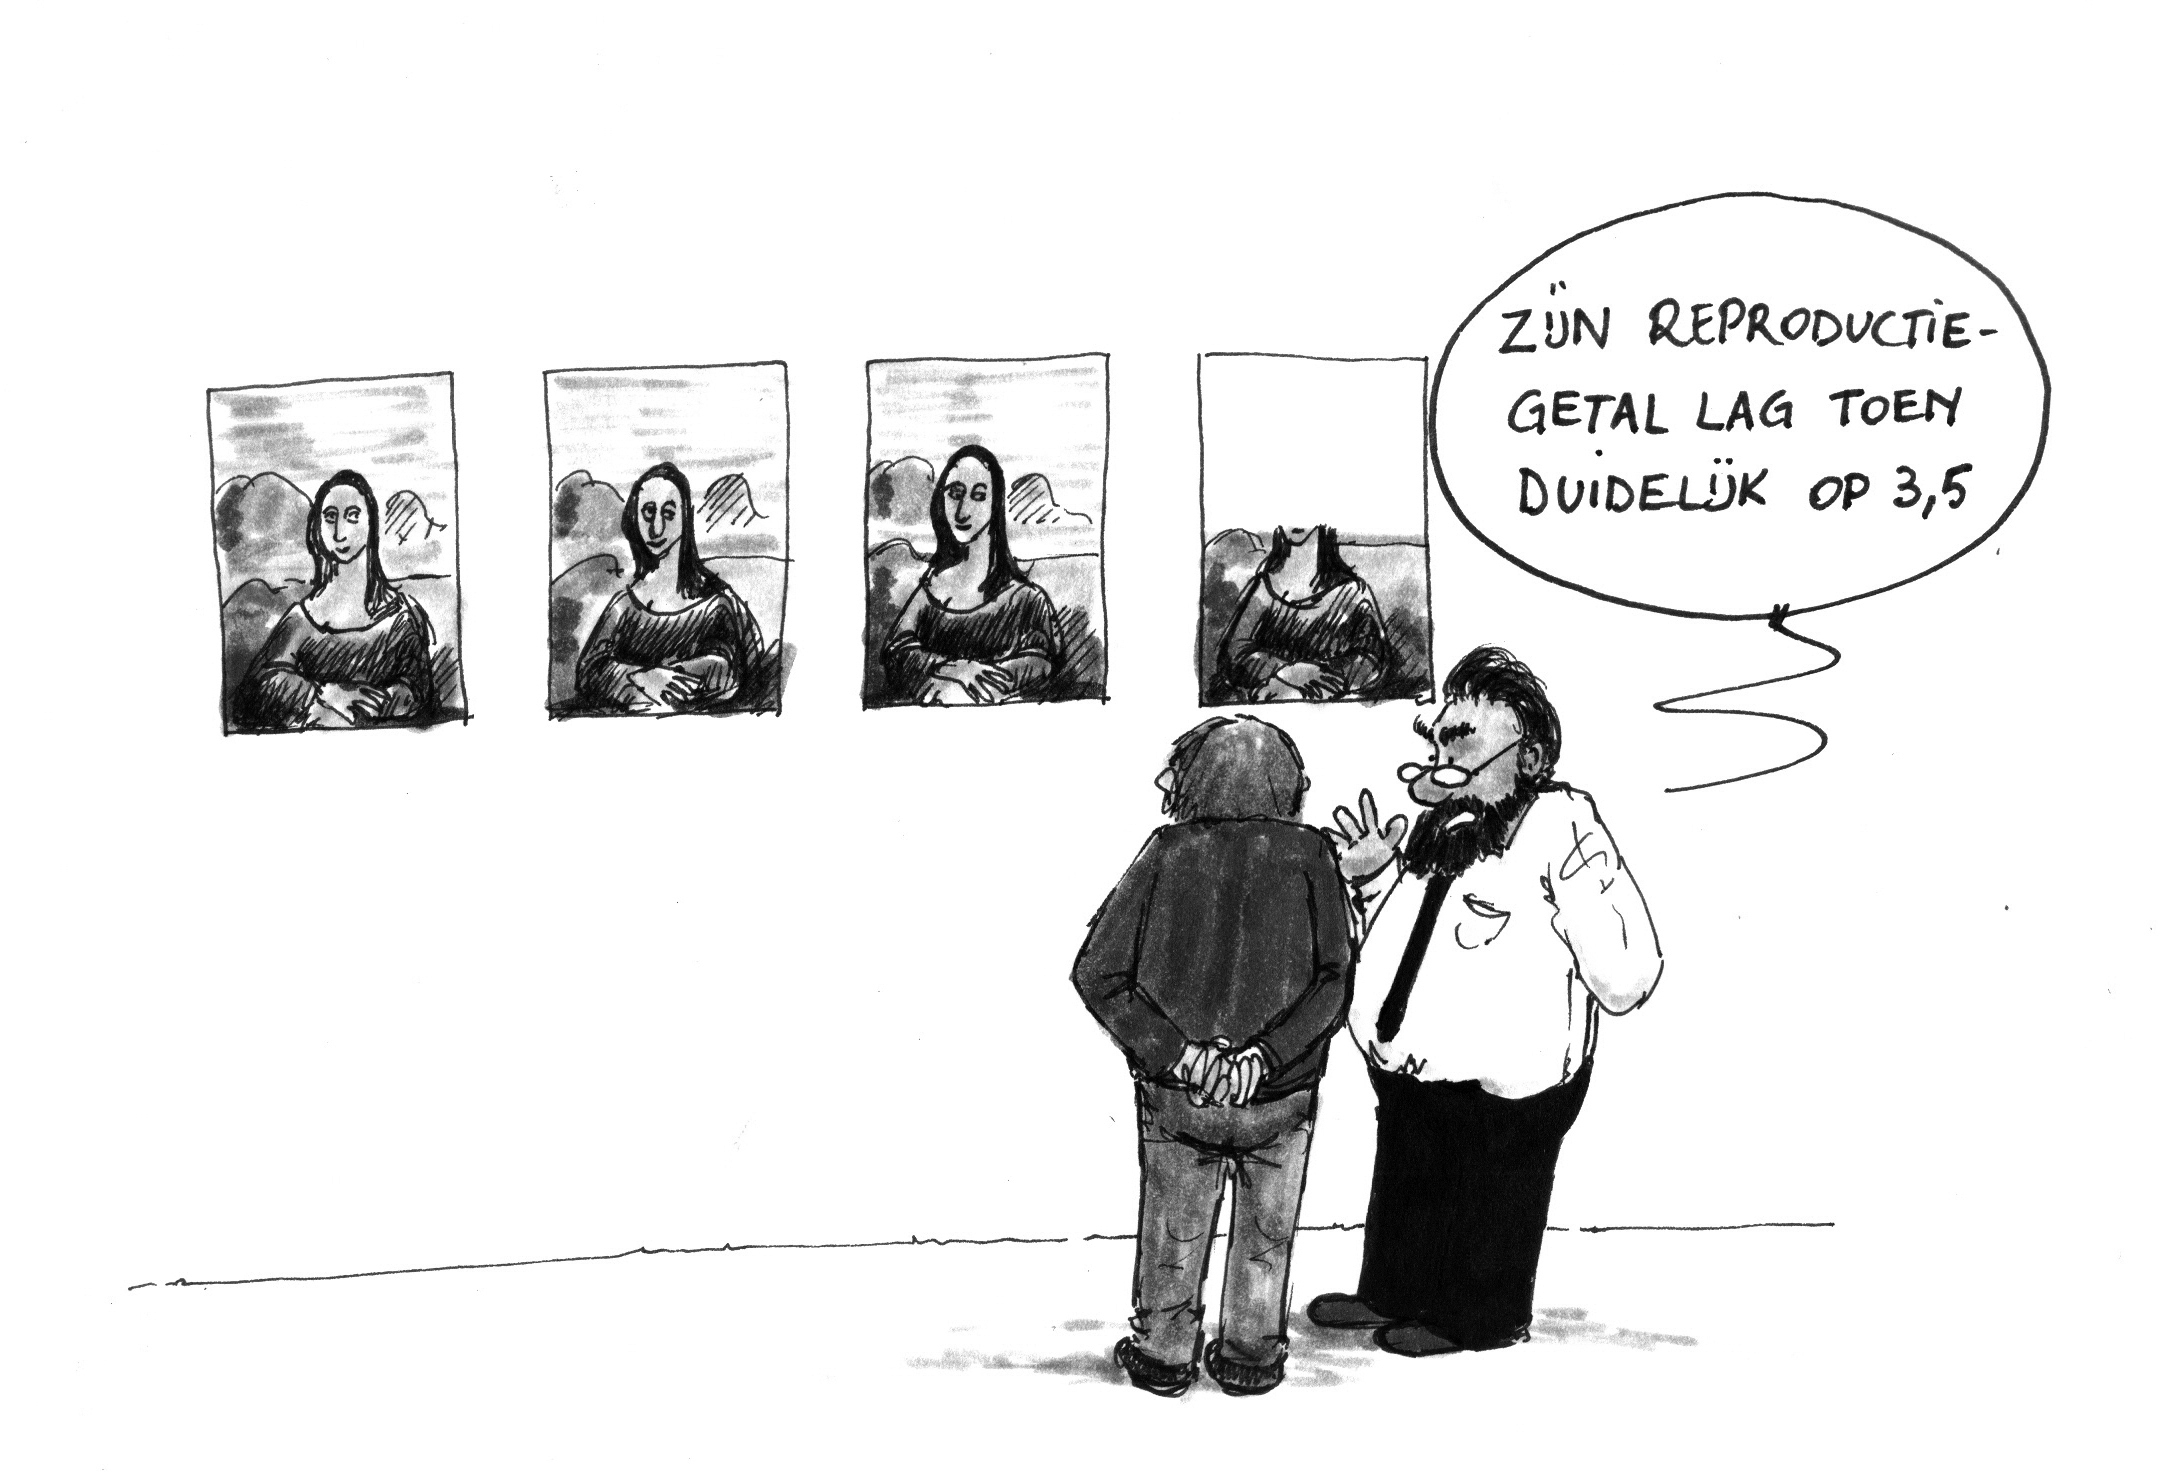
\includegraphics[width=14cm]{img/reproductiegetal.jpg}
\end{center}
\end{figure}

Met de gegevens uit de derde vaststelling vinden we dat de overgangsfunctie bereikt wordt als de besmettingsgraad gelijk is aan
\[b=\frac{\frac{1}{60}}{\frac{99}{100}}=\frac{1}{59,4}.\]
Een besmettingsgraad $b=\frac{1}{59}$ geeft dus een epidemie, een besmettingsgraad $b=\frac{1}{60}$ geeft een uitdovend ziektepatroon. Een minuscule verandering in de besmettingsgraad kan dus zorgen voor een uitdoving of voor een heropflakkeren van de ziekte. Zulke plotse verandering in de output door een kleine verandering in de input wordt wel eens het \emph{vlindereffect} (\emph{butterfly effect}) genoemd.

\eindewerktekst



\begin{multicols}{2}

\subsection{Keuzes bij het onderzoek}

De keuzes die we maakten voor dit project waren voornamelijk ingegeven door de voorkennis van de leerlingen, maar ook door enkele noden uit het hoger onderwijs.

\tussentitel{Een discreet model of een continu?}

In UW36/3 publiceerde Walter Van Assche een spinnenwebbijdrage over het SIR-model waarbij hij differentiaalvergelijkingen gebruikte. Vele bronnen formuleren het SIR-model met continue functies en differentiaalvergelijkingen. 

Mijn collega en ik werkten met leerlingen van het vijfde en het zesde jaar. Omdat de leerlingen van het vijfde nog maar net begonnen waren met het begrip afgeleide, formuleerden we dit model als een discreet model. Differentiaalvergelijkingen werden differentievergelijkingen. Differenties kwamen reeds eerder aan bod in de lessen analyse. De drie grafieken van het VAN-model werden getrapte grafieken, die elke kwartdag een sprongetje namen. Voor de leerlingen was het duidelijk dat de sprongen elkaar ook sneller konden opvolgen, bijvoorbeeld per uur, per minuut of per seconde. De link naar het continue model was hiermee gemaakt.

\end{multicols}


\begin{multicols}{2}

We merken op dat de voorspellingen van het SIR-model beduidend beïnvloed worden door de gekozen stapgrootte (Spons, 2018). Bij kleine stapgrootten zit er echter niet zoveel verschil meer op de resultaten. Vandaar dat we een redelijk kleine stapgrootte kozen voor dit project: een kwartdag.




\tussentitel{Een rekenblad of programmeren?}

De grafieken van de V-functie, de A-functie en de N-functie kunnen makkelijk gemaakt worden in een rekenblad. Hiervoor zijn drie kolommen nodig met getallen waarvan de formules gewoon per kwartdag doorgesleept kunnen worden. Echter, bij grote tabellen of bij het vergelijken van verschillende infectiegrafieken wordt een rekenblad log. Door te programmeren kan een simulatie compacter uitgevoerd worden.

De meeste van mijn leerlingen hadden nog nooit geprogrammeerd. Ik had samen met mijn collega een snelcursus programmeren in COCALC opgesteld. De cursus focuste alleen op de items die de leerlingen nodig zouden hebben voor het VAN-project: het maken en bewerken van lijsten, het opstellen van for-lussen, het afdrukken van meervoudige grafieken, het invoegen van verklarende teksten in html, het werken met sliders ... Het verbaasde me maar geen van de leerlingen had moeite met de programmeertaal. 

\tussentitel{Waarom CoCalc?}

CoCalc is een gratis platform dat gebaseerd is op de programmeertaal Sage, een neefje van Python. Pythonachtige talen hebben door hun eenvoud de reputatie geschikt te zijn voor een eerste kennismaking met het programmeren. CoCalc heeft een grote rekenkracht en levert mooie grafieken af. 

Bovendien kun je van een CoCalc-programma makkelijk een verslag maken. Je voegt tussen de programmablokken tekstblokken toe, klikt de programmaregels weg en laat de output van de programmaregels staan. Zo wordt het geheel leesbaar voor geïnteresseerden die geen aandacht willen besteden aan de programmatuur.

Tekstblokjes worden geschreven in html, de wereldwijde standaard voor webteksten. Het is interessant voor leerlingen hier kennis mee te maken. Formules worden geschreven in LaTeX, de wereldwijde standaard voor wetenschappelijke teksten. Ook een kennismaking met LaTeX is zinvol in richtingen met een wiskundige of wetenschappelijke component.
\newpage


\section{Eindbeschouwing}
Er zijn zeer veel wiskundige facetten aan epidemiologie. We toonden er slechts enkele: het meten van de clustervorming binnen een populatie, de sensitiviteit en de specificiteit van een besmettingstest en het ombuigen van de besmettingsgrafiek. Maar er zijn er nog. Denken we bijvoobeeld aan het nut van het mengen van speekselstalen wanneer bijvoorbeeld alle klassen van een school snel moeten gecontroleerd worden op een besmetting.

Voor leerkrachten wiskunde is het interessant iets af te weten van deze toepassingen. Door de link te leggen met recente maatschappelijke problemen, win je de interesse van heel wat leerlingen. Maakte je vorig jaar nog kansbomen in de context van lottoballetjes die getrokken worden zonder teruglegging, dan is het nu de moeite om bomen te maken over de PCR-test of de CT-test. Stellen de leerlingen je de vraag hoe het zit met het reproductiecijfer van een epidemische ziekte, dan kan je rustig het verschil uitleggen tussen een reproductiegetal groter en kleiner dan 1 door te verwijzen naar de infectiegrafieken van een uitdovende en een woekerende ziekte.

Het verhaal van de corona-epidemie is nog niet ten einde. Over een jaar hebben we weer nieuwe inzichten over epidemische ziekten. En hopelijk brengen die ook nieuwe wiskundige modellen met zich mee. We houden je op de hoogte.

\end{multicols}


\stopcontents[mainsections]			        % altijd laten staan, opsomming in inhoudstafel enkel tot loep beperken


% bronnen toevoegen
\begin{bronnen}
\item Bai, H., Hsieh, B., et al. (2020). \textit{Performance of radiologists in differentiating Covid-19 from viral pneumonia on chest CT}. Radiological Society of North America.
\item Developing and deploying tests for SARS-CoV-2 is crucial. \emph{The Economist} (2020, March 2th).
\item Dewatripont, M., Goldman, M., et al. (2020). Rapidly identifying workers who are immune to Covid-19 and virus-free is a priority for restarting the economy. \emph{VOX EU}.
\item John Hopkins Center for Health Security (2020). \textit{Serology-based tests for Covid-19}.
\item Medow, M., Lucey, C. (2011). A qualitative approach to Bayes' theorem. \emph{BMJ Evidence-Based Medicine 16}, 163-167.
\item Moons, F. (2020). Wiskunde \& Corona: Waarom we best een pact sluiten met onze 4 vertrouwelingen. \emph{Knack.be}.
\item Moons, F., \& Vandervieren, E. (2020). Wiskunde \& Corona: Waarom iedereen testen geen goed idee is. \emph{Knack.be}.
\item Spons, T. (2018). \emph{Een bijdrage aan de cursus Wiskundige methoden voor biomedische wetenschappen}, (niet gepubliceerde masterproef).KU Leuven. \item Van Assche, W. (2020).Wiskundige achtergrond bij de coronacrisis. \emph{Uitwiskeling 36/3}, 3-5.
\item https://nl.wikipedia.org/wiki/Reproductiegetal. Geraadpleegd op 15 juli 2020.
\end{bronnen}

